<<<<<<< HEAD
\begin{name}
	{\tenchude}
	{THPT Thiệu Hóa, Thanh Hóa}
	{LỚP TOÁN THẦY PHÁT}
	{ Với một người luôn biết cố gắng, không có gì là không thể}
\end{name}

\TN
\setcounter{ex}{0}
\Opensolutionfile{ans}[ans/ans-TT-ThieuHoa-ThanhHoa-L1-25-26]
%Câu 1
\begin{ex}%[Duong Xuan Loi]%[1H8N4-3]
	Cho hình chóp $S.ABC$ có $SA\perp(ABC)$ và $AB\perp BC$. Góc giữa hai mặt phẳng $(SBC)$ và $(ABC)$ là góc nào sau đây?		
	\choice
	{$\widehat{SIA}$ với $I$ là trung điểm của $BC$}
	{\True $\widehat{SBA}$}
	{$\widehat{SCB}$}
	{$\widehat{SCA}$}
	\loigiai{
		\immini[thm]{
			Ta có $\heva{&(SBC) \cap (ABC) = BC \\ &AB \subset (ABC), SB \subset (SBC) .}$\\
			Mặt khác
			\begin{itemize}
				\item $AB \perp BC$ (giả thiết).
				\item $SA \perp (ABC) \Rightarrow SA \perp BC$.
			\end{itemize}
			Suy ra $BC \perp (SAB) \Rightarrow BC \perp SB$.\\
			Vậy $\left((SBC),(ABC)\right)=(SB,AB)=\widehat{SBA}$ (vì $\triangle SAB$ vuông tại $A$).
		}{
			\begin{tikzpicture}[scale=0.8, font=\footnotesize, line join=round, line cap=round,>=stealth]
				\path
				(0,0) coordinate (A)
				(1.5,-1.2) coordinate (B)
				(4,0) coordinate (C)
				($(A)+(0,3.0)$) coordinate (S)	
				;
				\draw (S)--(A)--(B)--(C)--cycle (S)--(B);	
				\draw[dashed] (A)--(C);	
				\foreach \p/\q in {S/90,A/180,B/-90,C/0}
				\fill[black] (\p) circle (1.0pt) ($(\p)+(\q:3mm)$) node{$\p$};
				\draw pic[draw, angle radius=2mm] {right angle = S--A--B};
				\draw pic[draw, angle radius=2mm] {right angle = A--B--C};
			\end{tikzpicture}
		}
	}
\end{ex}
\begin{ex}%[Duong Xuan Loi]%[2H2N1-1]
	Cho hình lăng trụ $ABC.A'B'C'$, $M$ là trung điểm của $BB'$. Đặt $\overrightarrow{CA}=\overrightarrow{a}$, $\overrightarrow{CB}=\overrightarrow{b}$, $\overrightarrow{AA'}=\overrightarrow{c}$. Khẳng định nào sau đây đúng?
	\choice
	{\True $\overrightarrow{AM}=\overrightarrow{b}-\overrightarrow{a}+\dfrac{1}{2}\overrightarrow{c}$}
	{$\overrightarrow{AM}=\overrightarrow{a}+\overrightarrow{c}-\dfrac{1}{2}\overrightarrow{b}$}
	{$\overrightarrow{AM}=\overrightarrow{b}+\overrightarrow{c}-\dfrac{1}{2}\overrightarrow{a}$}
	{$\overrightarrow{AM}=\overrightarrow{a}-\overrightarrow{c}+\dfrac{1}{2}\overrightarrow{b}$}
	\loigiai{
		\immini[thm]{
			Ta có $\overrightarrow{AM} = \overrightarrow{AB} + \overrightarrow{BM} = \left( \overrightarrow{CB} - \overrightarrow{CA} \right) + \dfrac{1}{2}\overrightarrow{BB'}$.\\
			Mặt khác $\overrightarrow{BB'} = \overrightarrow{AA'}$.\\
			Suy ra $\overrightarrow{AM} = \overrightarrow{b} - \overrightarrow{a} + \dfrac{1}{2}\overrightarrow{c}$.
		}{
			\begin{tikzpicture}[scale=0.7, font=\footnotesize, line join=round, line cap=round,>=stealth]
				\path
				(0,0)coordinate (A)
				(1.1,-1.5)coordinate (B)
				(4,-0.5)coordinate (C)
				($(A)+(0,3.8)$) coordinate (A')
				($(A')+(B)-(A)$)coordinate (B')
				($(A')+(C)-(A)$)coordinate (C')		
				($(B')!0.5!(B)$) coordinate (M)					
				;
				\draw (A)--(B)--(C)--(C')--(B')--(A')--cycle (A')--(C') (B)--(B') (A)--(M);
				\draw[dashed] (A)--(C);	
				\foreach \p/\q in {A/180,B/-90,C/0,A'/180,B'/70,C'/0,M/0}
				\fill[black] (\p) circle (1.0pt)node[shift={(\q:3mm)}]{$\p$};
			\end{tikzpicture}
	}}
\end{ex}

\begin{ex}%[Duong Xuan Loi]%[1D6N4-2]
	Tích các nghiệm của phương trình $2^{x^2-2x}=8$ là
	\choice
	{$2$}
	{$0$}
	{$3$}
	{\True $-3$}
	\loigiai{
		Ta có \[2^{x^2-2x}=8\Leftrightarrow 2^{x^2-2x}=2^3\Leftrightarrow x^2-2x=3\Leftrightarrow x^2-2x-3=0\Leftrightarrow \hoac{& x= -1\\ & x=3.}\]
		Tích các nghiệm của phương trình là $(-1)\cdot3=-3$.
	}
\end{ex}

\begin{ex}%[Duong Xuan Loi]%[2D1N2-1]
	Cho hàm số $f(x)$ có đạo hàm $f'(x)=(x+1)x^2(x-3)^3$, $\forall x\in\mathbb{R}$. Hàm số đã cho có bao nhiêu điểm cực trị?
	\choice
	{$3$}
	{\True $2$}
	{$5$}
	{$1$}
	\loigiai{
		Ta có $f'(x)=0\Leftrightarrow\hoac{&x=-1 \text{ (nghiệm bội lẻ)}\\& x=0 \text{ (nghiệm bội chẵn)}\\ & x=3 \text{ (nghiệm bội lẻ)}.}$\\
		Bảng xét dấu
		\begin{center}
			\begin{tikzpicture}
				\tkzTabInit[nocadre=false,lgt=1.2,espcl=2.5,deltacl=0.6]
				{$x$ /0.6, $f'(x)$ /0.6, $f(x)$ /2.5}
				{$-\infty$,$-1$,$0$,$3$,$+\infty$}
				\tkzTabLine{,+,$0$,-,$0$,-,$0$,+,}
				\tkzTabVar{-/,+/CĐ,R,-/CT,+/$+\infty$}
			\end{tikzpicture}
		\end{center}
		Từ bảng xét dấu suy ra hàm số có $2$ cực trị.		
	}
\end{ex}

\begin{ex}%[Thi thử, THPT Thiệu Hóa, Thanh Hóa, 2026]%[Thành Đức Trung]%[1D3V2-7]
	Cho hai đồ thị $y = \dfrac{1}{x}$ và $y = \sqrt{x}$ cắt nhau tại điểm $A(1;1)$. Với số thực $t>1$, đường thẳng $y=t$ lần lượt cắt đồ thị $y = \dfrac{1}{x}$ và $y=  \sqrt{x}$ tại các điểm $B$ và $C$.
	\begin{center}
		\begin{tikzpicture}[scale=1.3, font=\normalsize, >=stealth]  
			\draw[->] (-1,0)--(0,0) node[below left]{$O$}--(7,0) node[below]{$x$};
			\draw[->] (0,-1) --(0,3.5) node[right]{$y$};
			\draw [black,thick, domain=0:5.5, samples=100] plot(\x,{sqrt((\x))}) node[above]{$y = \sqrt{x}$};
			\draw [black,thick, domain=0.35:5, samples=100] plot(\x,{1/(\x)}) node[right]{$y = \tfrac{1}{x}$};
			\draw[fill = black] (0,0) circle (1pt);
			\draw (-1,2)--(6,2) node[below] {$y=t$} (4,-1)--(4,3);
			\path 
			(1,1) coordinate (A)
			(.5,2) coordinate (B)
			(4,2) coordinate (C)
			(4,.25) coordinate (D)
			;
			\draw[dashed] (1,0) node[below]{$1$} -- (A) -- (0,1) node[left]{$1$};
			\draw (A)--(B)--(C)--(A)--(D)--(C);
			\fill[color=blue,opacity=.2] (A)--(B)--(C)--(A);
			\fill[color=red,opacity=.2] (A)--(D)--(C)--(A);
			\foreach \x/\g in{A/80, B/60, C/-45, D/45}
			\fill[black](\x)circle(1pt)($(\x)+(\g:2.5mm)$)node{$\x$};
		\end{tikzpicture}
	\end{center}
	Từ $C$ kẻ đường thẳng song song với trục $Oy$, cắt đồ thị $y = \dfrac{1}{x}$ tại điểm $D$. Gọi $f(t)$ là diện tích tam giác $ACB$ và $g(t)$ là diện tích tam giác $ADC$. Tính $L = \displaystyle\lim_{t\to1^+}\dfrac{g(t)}{f(t)}$.
	\choice
	{$L = +\infty$}
	{$L = \dfrac{5}{3}$}
	{$L = 0$}
	{\True $L = 2$}
	\loigiai
	{
		Vì $B$ là giao điểm của hai đồ thị hàm số $y=t$ và $y=\dfrac{1}{x}$ nên $B\left(\dfrac{1}{t};t\right)$. \\
		Vì $C$ là giao điểm của hai đồ thị hàm số $y=t$ và $y=\sqrt{x}$ nên $C\left(t^2;t\right)$. \\
		Đường thẳng đi qua $C$ và song song với $Oy$ có phương trình là $x=t^2$. \\
		Vì $D$ là giao điểm của hai đồ thị hàm số $y=\dfrac{1}{x}$ và $x=t^2$ nên $D\left(t^2;\dfrac{1}{t^2}\right)$. \\
		Xét $\triangle ABC$ có
		\[f(t) = S_{\triangle ABC} = \dfrac{1}{2}BC\cdot\mathrm{d}\left(A,BC\right) = \dfrac{1}{2}\cdot \left(t^2-\dfrac{1}{t}\right)\cdot \left(t - 1\right) = \dfrac{\left(t^3-1\right)(t-1)}{2t}.\]
		Xét $\triangle ADC$ có
		\[g(t) = S_{\triangle ADC} = \dfrac{1}{2}CD\cdot\mathrm{d}\left(A,CD\right) = \dfrac{1}{2}\cdot \left(t - \dfrac{1}{t^2}\right)\cdot \left(t^2 - 1\right) = \dfrac{\left(t^3-1\right)\left(t^2-1\right)}{2t^2}.\]
		Suy ra $L = \displaystyle\lim_{t\to1^+}\dfrac{g(t)}{f(t)} = \displaystyle\lim_{t\to1^+} \dfrac{t^2-1}{t(t-1)} = 2$.
	}
\end{ex}

%%%% Câu 6
\begin{ex}%[Thi thử, THPT Thiệu Hóa, Thanh Hóa, 2026]%[Thành Đức Trung]%[0D1N2-2] 
	Số tập con của tập hợp gồm $2\,026$ phần tử là
	\choice
	{$2 \times 2026$}
	{$2026$}
	{$2026^2$}
	{\True $2^{2026}$}
	\loigiai
	{
		Số tập con của một tập hợp có $n$ phần tử là $2^n$. \\
		Với $n = 2\,026$, số tập con của tập hợp đã cho là $2^{2\,026}$.
	}
\end{ex}

%%%% Câu 7
\begin{ex}%[Thi thử, THPT Thiệu Hóa, Thanh Hóa, 2026]%[Thành Đức Trung]%[2H2V2-2]
	Trong không gian $Oxyz$, cho hai điểm $A(1;2;1)$, $B(2;-1;3)$ và điểm $M(a;b;0)$ sao cho $MA^2 + MB^2$ nhỏ nhất. Giá trị của $a+b$ là
	\choice
	{$3$}
	{$-2$}
	{$1$}
	{\True $2$}
	\loigiai
	{
		Gọi $I$ là trung điểm của đoạn thẳng $AB$ suy ra $I\left( \dfrac{3}{2}; \dfrac{1}{2}; 2 \right)$.\\
		Khi đó $MA^2 + MB^2 = \left(\overrightarrow{MI} + \overrightarrow{IA}\right)^2 + \left(\overrightarrow{MI} + \overrightarrow{IB}\right)^2 = 2MI^2 + IA^2 + IB^2$ (do $\overrightarrow{IA} + \overrightarrow{IB} = \overrightarrow{0}$).\\
		Để $MA^2 + MB^2$ nhỏ nhất thì $MI$ nhỏ nhất. Mà $M(a;b;0) \in (Oxy)$, do đó $M$ là hình chiếu vuông góc của $I$ trên mặt phẳng $(Oxy)$.\\
		Suy ra $M\left( \dfrac{3}{2}; \dfrac{1}{2}; 0 \right)$, tức là $a = \dfrac{3}{2}$ và $b = \dfrac{1}{2}$.\\
		Vậy $a + b = \dfrac{3}{2} + \dfrac{1}{2} = 2$.
	}
\end{ex}

%%%% Câu 8
\begin{ex}%[Thi thử, THPT Thiệu Hóa, Thanh Hóa, 2026]%[Thành Đức Trung]%[2H2N2-2]
	Trong không gian với hệ tọa độ $Oxyz$, cho hai điểm $A(-3;4;5)$, $B(-1;0;1)$. Tìm tọa độ điểm $M$ thỏa mãn $\overrightarrow{MA} + \overrightarrow{MB} = \overrightarrow{0}$.
	\choice
	{$M(-4;-4;-4)$}
	{$M(4;4;4)$}
	{\True $M(-2;2;3)$}
	{$M(1;2;3)$}
	\loigiai
	{
		Điều kiện $\overrightarrow{MA} + \overrightarrow{MB} = \overrightarrow{0}$ tương đương với $M$ là trung điểm của đoạn thẳng $AB$.\\
		Tọa độ điểm $M$ là
		$\heva{&x_M = \dfrac{x_A + x_B}{2} = \dfrac{-3 + (-1)}{2} = -2 \\ &y_M = \dfrac{y_A + y_B}{2} = \dfrac{4 + 0}{2} = 2 \\ &z_M = \dfrac{z_A + z_B}{2} = \dfrac{5 + 1}{2} = 3.}$\\
		Vậy $M(-2;2;3)$.
	}
\end{ex}


\begin{ex}%[TT-ThieuHoa-ThanhHoa-L1-25-26]%[Vũ Nguyễn Hoàng Anh]%[1D2H3-4]
	Diện tích rừng tự nhiên của nước ta năm $2\,021$ là xấp xỉ $10\,171\,757$ ha. 
	Giả sử tỉ lệ tăng diện tích rừng tự nhiên hằng năm kể từ năm $2\,021$ là $0{,}7\%$/năm. 
	Diện tích rừng tự nhiên của nước ta vào năm $2\,025$ xấp xỉ bằng
	\choice
	{$10\,468\,251$ ha}
	{\True $10\,459\,571$ ha}
	{$10\,386\,863$ ha}
	{$10\,532\,788$ ha}
	\loigiai{
		 Diện tích rừng của nước ta vào năm $2\,025$ xấp xỉ $10\,171\,757(1+0{,}7\%)^4\approx 10\,459\,571$ ha.
	}
\end{ex}

\begin{ex}%[TT-ThieuHoa-ThanhHoa-L1-25-26]%[Vũ Nguyễn Hoàng Anh]%[2D1N1-2]
	\immini[thm]{
		Cho hàm số $y=f(x)$ có đồ thị như hình vẽ.  
	Hãy chọn đáp án đúng.
	\choice
	{Hàm số nghịch biến trên $(0;2)$}
	{Hàm số đồng biến trên $(-\infty;0)$ và $(2;+\infty)$}
	{Hàm số đồng biến trên $(-1;0)$ và $(2;3)$}
	{\True Hàm số nghịch biến trên $(-\infty;0)$ và $(2;+\infty)$}
	}{
		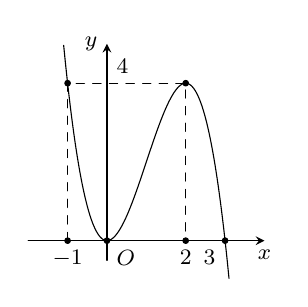
\begin{tikzpicture}[line cap=round, line join=round,font=\footnotesize,>=stealth, scale=0.5]
			\tikzset{label style/.style={font=\footnotesize}}
			\draw[->] (-2,0)--(4,0)node[below]{$x$};
			\draw[->] (0,-0.5)--(0,5) node[left]{$y$};
			\draw[dashed] (-1,0)node[below]{$-1$}--(-1,4)--(0,4) node[above right]{$4$}--(2,4)--(2,0) node[below]{$2$};
			\draw[fill=black] (0,0) circle (2pt) node[below right]{$O$}
			(3,0) circle (2 pt) node[below left]{$3$}
			(-1,0) circle (2pt)
			(2,0) circle (2pt)
			(-1,4) circle (2pt)
			(2,4) circle (2pt);
			\draw[smooth, samples=100] plot[domain=-1.1:3.1] (\x, { -(\x)^2*(\x-3) });
			
		\end{tikzpicture}
	}
	\loigiai{
		Dựa vào đồ thị hàm số, hàm số nghịch biến trên các khoảng $(-\infty;0)$ và $(2;+\infty)$.  
	}
\end{ex}

\begin{ex}%[TT-ThieuHoa-ThanhHoa-L1-25-26]%[Vũ Nguyễn Hoàng Anh]%[2H2H2-2] 
	Trong không gian với hệ trục tọa độ cho trước (đơn vị đo lấy theo kilmet), 
	ra đa phát hiện một máy bay di chuyển với vận tốc và hướng không đổi 
	từ điểm $A(750;450;7)$ đến điểm $B(950;550;9)$ trong $10$ phút.  
	Nếu máy bay tiếp tục giữ nguyên vận tốc và hướng bay trong $10$ phút nữa 
	đến điểm $C(x;y;z)$ thì $x+y+z$ bằng
	\choice
	{$1\,931$}
	{\True $1\,811$}
	{$1\,691$}
	{$1\,781$}
	\loigiai{
		Từ giả thiết, ta thấy $B$ là trung điểm $AC$, do đó $C=(1\,150;650;11)$. Từ đó $x+y+z= 1\,811$.
	}
\end{ex}

\begin{ex}%[TT-ThieuHoa-ThanhHoa-L1-25-26]%[Vũ Nguyễn Hoàng Anh]%[2D4N1-3] 
	Thời gian (phút) truy cập Internet mỗi buổi tối của một số học sinh được cho trong bảng sau
	\begin{center}
		\begin{tabular}{|c|c|c|c|c|c|}
			\hline
			Thời gian (phút) & $[9{,}5;12{,}5)$ & $[12{,}5;15{,}5)$ & $[15{,}5;18{,}5)$ & $[18{,}5;21{,}5)$ & $[21{,}5;24{,}5)$ \\
			\hline
			Số học sinh & $3$ & $12$ & $15$ & $24$ & $2$ \\
			\hline
		\end{tabular}
	\end{center}
	Khoảng tứ phân vị của mẫu số liệu ghép nhóm là
	\choice
	{$4{,}63$}
	{$10{,}75$}
	{$4{,}38$}
	{\True $4{,}75$}
	\loigiai{
		Ta có bảng
		\begin{center}
			\begin{tabular}{|c|c|c|c|c|c|}
				\hline
				Thời gian (phút) & $[9{,}5;12{,}5)$ & $[12{,}5;15{,}5)$ & $[15{,}5;18{,}5)$ & $[18{,}5;21{,}5)$ & $[21{,}5;24{,}5)$ \\
				\hline
				Số học sinh & $3$ & $12$ & $15$ & $24$ & $2$ \\
				\hline
				Tần số tích lũy & $3$ &$15$ & $30$ &$54$&$56$\\
				\hline 
			\end{tabular}
		\end{center}
		Suy ra $Q_1=12{,}5+\dfrac{3\left(\dfrac{56}{4}-3\right)}{12}=15{,}25$, $Q_3=18{,}5+\dfrac{3\left(\dfrac{3\cdot 56}{4}-30\right)}{24}=20$. Vậy khoảng tứ phân vị của mẫu số liệu là $\Delta Q=Q_3-Q_1=4{,}75$.	}
\end{ex}


\cauds

\begin{ex}%[Duong Xuan Loi]%[2D1H5-3]
	Cho hàm số $y=f(x)$ có bảng biến thiên như sau
	\begin{center}
		
\begin{tikzpicture}
			\tkzTabInit[nocadre=false,lgt=1.2,espcl=2.5,deltacl=0.6]
			{$x$ /0.6, $f'(x)$ /0.6, $f(x)$ /2.5}
			{$-\infty$,$-1$,$1$,$+\infty$}
			\tkzTabLine{,+,$0$,-,$0$,+,}
			\tkzTabVar{-/$-\infty$,+/$3$,-/$-1$,+/$+\infty$}
		\end{tikzpicture}
	\end{center}
	Các mệnh đề sau đúng hay sai?
	\choiceTF
	{\True $f'(x)=0\Leftrightarrow\hoac{&x=-1\\&x=1}$}
	{\True Đồ thị hàm số $y=f(x)$ cắt trục $Ox$ tại $3$ điểm phân biệt}
	{Giá trị cực tiểu của hàm số bằng $1$}
	{\True Hàm số $y=f(2-x)$ đồng biến trên $(1;3)$}
	\loigiai{
		\begin{itemchoice}
			\itemch Ta có $f'(x)=0\Leftrightarrow\hoac{&x=-1\\&x=1.}$		
			\itemch Ta có $y_{\text{CĐ}}\cdot y_{\text{CT}}=3\cdot(-1)=-3<0$ suy ra đồ thị hàm số $y=f(x)$ cắt trục $Ox$ tại $3$ điểm phân biệt.
			\itemch Ta có $y_{\text{CT}}=-1$.
			\itemch Xét hàm số $y=f(2-x)$.\\
			Có $y'=-f'(2-x)$.\\
			$y'=0\Leftrightarrow f'(2-x)=0\Leftrightarrow \hoac{& 2-x=-1 \\ & 2-x=1}\Leftrightarrow\hoac{& x=3 \\ & x=1.}$\\
			Bảng xét dấu
			\begin{center}
				
\begin{tikzpicture}
					\tkzTabInit[nocadre=false,lgt=1.2,espcl=2.5,deltacl=0.6]
					{$x$ /0.6, $y'$ /0.6, $y$ /2.5}
					{$-\infty$,$1$,$3$,$+\infty$}
					\tkzTabLine{,-,$0$,+,$0$,-,}
					\tkzTabVar{+/,-/,+/,-/}
				\end{tikzpicture}
			\end{center}
			Từ bảng xét dấu suy ra hàm số đồng biến trên $(1;3)$.
		\end{itemchoice}
	}
\end{ex}

\begin{ex}%[Thi thử, THPT Thiệu Hóa, Thanh Hóa, 2026]%[Thành Đức Trung]%[2D3H2-3]
	Thời gian hoàn thành một bài viết chính tả của một số học sinh lớp $4$ hai trường X và Y được ghi lại ở bảng sau
	\begin{center}
		\begin{tabular}{|c|c|c|c|c|c|}
			\hline
			Thời gian (phút)	& $\left[ 6;7 \right)$ & $\left[ 7;8 \right)$ & $\left[ 8;9 \right)$ & $\left[ 9;10 \right)$ & $\left[ 10;11 \right)$ \\
			\hline
			Số học sinh trường X	& $8$ & $10$ & $13$ & $10$ & $9$ \\
			\hline
			Số học sinh trường Y	& $4$ & $12$ & $17$ & $14$ & $3$ \\
			\hline
		\end{tabular}
	\end{center}
	\choiceTF
	{\True Nếu so sánh theo độ lệch chuẩn thì học sinh trường Y có tốc độ viết đồng đều hơn}
	{Nếu so sánh theo khoảng tứ phân vị thì học sinh trường X có tốc độ viết đồng đều hơn}
	{Phương sai của mẫu số liệu ghép nhóm của trường X là $1{,}08$ và phương sai của mẫu số liệu ghép nhóm của trường Y là $1{,}7584$}
	{\True Nếu so sánh theo số trung bình thì học sinh trường Y viết nhanh hơn}
	\loigiai
	{
		Với trường X, tổng số học sinh
		\[
		n_X = 8+10+13+10+9 = 50.
		\]
		\begin{itemize}
			
			\item {Số trung bình}
			\[
			\overline{x}_X
			= \dfrac{8\cdot6{,}5 + 10\cdot7{,}5 + 13\cdot8{,}5 + 10\cdot9{,}5 + 9\cdot10{,}5}{50}
			= 8{,}54\ (\text{phút}).
			\]
			\item {Khoảng tứ phân vị}
			\[
			Q_{1X} = 7 + \dfrac{12{,}5 - 8}{10}\cdot 1 = 7{,}45.
			\]
			\[
			Q_{3X} = 9 + \dfrac{37{,}5 - 31}{10}\cdot 1 = 9{,}65.
			\]
			\[
			\Delta Q_X = 2{,}2.
			\]
			
			\item {Phương sai và độ lệch chuẩn}
			\[
			s_X^2 = \dfrac{1}{50}\sum n_i(x_i-\overline{x}_X)^2 = 1{,}7584,
			\qquad
			s_X =\sqrt{1{,}7854} = 1{,}33.
			\]
			
		\end{itemize}
		Với trường Y, tổng số học sinh
		\[
		n_Y = 4+12+17+14+3 = 50.
		\]
		\begin{itemize}
			\item {Số trung bình}
			
			\[
			\overline{x}_Y
			= \dfrac{4\cdot6{,}5 + 12\cdot7{,}5 + 17\cdot8{,}5 + 14\cdot9{,}5 + 3\cdot10{,}5}{50}
			= 8{,}50\ (\text{phút}).
			\]
			
			\item {Khoảng tứ phân vị}
			\[
			Q_{1Y} = 7 + \dfrac{12{,}5 - 4}{12}\cdot 1 \approx 7{,}71.
			\]			
			\[
			Q_{3Y} = 9 + \dfrac{37{,}5 - 33}{14}\cdot 1 \approx 9{,}32.
			\]
			\[
			\Delta Q_Y \approx 1{,}61.
			\]
			\item {Phương sai và độ lệch chuẩn}
			
			\[
			s_Y^2 = \dfrac{1}{50}\sum n_i(x_i-\overline{x}_Y)^2 \approx 1{,}08,
			\qquad
			s_Y \approx \sqrt{1{,}08} = 1{,}03.
			\]
			
		\end{itemize}
	}
\end{ex}

%%%% Câu 15
\begin{ex}%[Thi thử, THPT Thiệu Hóa, Thanh Hóa, 2026]%[Thành Đức Trung]%[1H8C7-9]
	\immini[thm]{Kim tự tháp Cheops là kim tự tháp lớn nhất trong các kim tự tháp ở Ai Cập, được xây dựng vào thế kỉ thứ $26$ trước Công nguyên và là một trong bảy kì quan của thế giới cổ đại. Kim tự tháp có dạng hình chóp $S.ABCD$ với đáy là hình vuông $ABCD$ tâm $H$ và cạnh đáy dài $262\,$m, các cạnh bên bằng nhau và dài $230\,$m (kích thước hiện nay).}{	
		\begin{tikzpicture}[line join = round,scale=0.7,xscale=0.7,yscale=1.2]
			\definecolor{vang}{HTML}{f2e6bc}
			\path (-3, 0.2) coordinate (A) -- (0, 0) coordinate (B) -- (2, 4) coordinate (C)
			(8, 0.1) coordinate (D);
			\path[inner color=vang,outer color=vang!60!white] (A)--(B)--(C)--cycle;
			\path[inner color=vang,outer color=vang!60!white] (D)--(B)--(C)--cycle;
			\foreach \i in {1,...,18}{
				\pgfmathsetmacro{\tiso}{\i/19}
				\draw[vang!65!orange,opacity=0.65] ($(B)!\tiso!(C)$)--($(B)!\tiso!(A)$);
				\draw[vang!65!orange,opacity=0.65]($(A)!\tiso!(C)$)--($(A)!\tiso!(B)$);
				\draw[vang!65!orange,opacity=0.65] ($(B)!\tiso!(C)$)--($(B)!\tiso!(D)$);
				\draw[vang!65!orange,opacity=0.65]($(D)!\tiso!(C)$)--($(D)!\tiso!(B)$);
			}
			\draw[black!65!gray] (B)--(D)--(C) (A)--(B)--(C)--cycle;
		\end{tikzpicture}
	}
	\noindent Biết căn phòng chứa đựng thông tin khảo cổ có dạng hình lập phương với thể tích $64\,$m$^3$ ngay tại trung tâm, có cạnh đáy song song với cạnh đáy của kim tự tháp và $H$ cũng là tâm của mặt sàn căn phòng. Các nhà khảo cổ muốn tạo một lỗ khoan từ bên ngoài vào căn phòng này.
	\choiceTF
	{\True Kim tự tháp có hình dạng là một hình chóp đều}
	{Chiều cao của kim tự tháp là $\sqrt{18\,579}\,$m}
	{\True Phần không gian mà kim tự tháp chiếm chỗ là $3\,118\,752\,$m$^3$ \textit{(làm tròn kết quả đến hàng đơn vị)}}
	{\True Chiều dài nhỏ nhất của lỗ khoan mà các nhà khảo cổ muốn tạo bằng $90$ mét \textit{(làm tròn kết quả đến hàng đơn vị)}}
	\loigiai
	{
		\begin{center}
			\begin{tikzpicture}[scale=0.9, font=\footnotesize, line join=round, line cap=round, >=stealth]
				\coordinate (A) at (2,2.5);
				\coordinate (B) at (0,0);
				\coordinate (C) at (6,0);
				\coordinate (D) at ($(A)+(C)-(B)$);
				\coordinate (H) at ($(A)!0.5!(C)$); % Giả sử H là hình chiếu của S
				\coordinate (S) at ($(H)+(0,5.5)$);
				\coordinate (M) at ($(C)!0.5!(D)$);
				\coordinate (F) at ($(S)!0.68!(M)$);
				\coordinate (A2) at ($(A)!0.65!(H)$); 
				\coordinate (B2) at ($(B)!0.65!(H)$);
				\coordinate (C2) at ($(C)!0.65!(H)$);
				\coordinate (D2) at ($(D)!0.65!(H)$);
				\coordinate (A1) at ($(A2)+(0,1.3)$);
				\coordinate (B1) at ($(B2)+(0,1.3)$);
				\coordinate (C1) at ($(C2)+(0,1.3)$);
				\coordinate (D1) at ($(D2)+(0,1.3)$);
				\coordinate (I) at ($(C1)!0.5!(D1)$);
				\draw[dashed] (S)--(A) (A)--(B) (A)--(D) (B)--(D) (A)--(C) (S)--(H) (H)--(M) (I)--(F);
				\draw (M)--(S)--(B) (S)--(C) (S)--(D) (B)--(C) (C)--(D);
				\draw[red, dashed, thick] (A1)--(B1)--(C1)--(D1)--cycle;
				\draw[red, dashed, thick] (A2)--(B2)--(C2)--(D2)--cycle;
				\draw[red, dashed, thick] (A1)--(A2) (B1)--(B2) (C1)--(C2) (D1)--(D2);
				\foreach \p/\pos in {S/above, A/left, B/left, C/right, D/right, H/below, M/below right, F/right, I/left}
				\fill[black] (\p) circle (1.5pt) node[\pos] {$\p$};
			\end{tikzpicture}\hspace*{1cm}
			\begin{tikzpicture}[>=stealth, scale=0.8, font=\footnotesize]
				\coordinate (S) at (0,6);
				\coordinate (H) at (0,0);
				\coordinate (M) at (4,0);
				\coordinate (N) at (1,0);
				\coordinate (I) at (1,1.5);
				\path ($(S)!(I)!(M)$) coordinate (F);
				\draw[dashed] (I)--(N);
				\draw (S)--(M) (I)--(F);
				\draw[->] (H)--($(S)+(0,0.5)$) node[left]{$y$};
				\draw[->] (H)--($(M)+(0.5,0)$) node[below]{$x$};
				\foreach\x/\y in {H/-135,N/-90,S/180,I/135,M/-90,F/40} \draw[fill=black] (\x) circle (1.2pt)+(\y:0.3) node{$\x$};
			\end{tikzpicture}
		\end{center}
		\begin{itemchoice}
			\itemch Vì đáy $ABCD$ là hình vuông và các cạnh bên bằng nhau nên $S.ABCD$ là hình chóp tứ giác đều.
			\itemch Ta có nửa đường chéo đáy là $AH = \dfrac{AC}{2} = \dfrac{262\sqrt{2}}{2} = 131\sqrt{2}\,$m. \\
			Chiều cao kim tự tháp là $h=SH = \sqrt{SA^2 - AH^2} = \sqrt{230^2 - \left(131\sqrt{2}\right)^2} = \sqrt{18\,578}\,$m.
			\itemch Thể tích kim tự tháp là $V = \dfrac{1}{3} \cdot S_{ABCD} \cdot SH = \dfrac{1}{3} \cdot 262^2 \cdot \sqrt{18\,578} \approx 3\,118\,752\,$m$^3$ (làm tròn đến hàng đơn vị).
			\itemch Để mũi khoan có chiều dài ngắn nhất, ta cần khoan từ mặt bên vào vị trí cạnh của khối lập phương. Khoảng cách ngắn nhất là khoảng cách từ một điểm $I$ thuộc cạnh trên của khối lập phương đến mặt bên của hình chóp.\\
			Gọi $M$ là trung điểm của cạnh $CD$, thì $HM=131$ m. Dựng hệ trục tọa độ $Oxy$ sao cho $H(0;0)$, $M(131;0)$, $S\left(0;h\right)$. Đường thẳng $SM$ có phương trình $\dfrac{x}{131}+\dfrac{y}{h}=1$.\\
			Do căn phòng có thể tích $64$ m$^3$ nên độ dài cạnh của phòng là $IN=4$ m. Suy ra $I(2;4)$. Vậy độ dài lỗ khoan nhỏ nhất là
			\[ \mathrm{d}(I,SM)=\dfrac{\left| \dfrac{2}{131}+\dfrac{4}{h}-1 \right|}{\sqrt{\dfrac{1}{131^2}+\dfrac{1}{h^2}}}\approx 90\text{ m}. \]
		\end{itemchoice}
	}
\end{ex}

\begin{ex}%[TT-ThieuHoa-ThanhHoa-L1-25-26]%[Vũ Nguyễn Hoàng Anh]%[2H2K2-6] 
	\immini[thm]{
		Trong hệ tọa độ $Oxyz$, đơn vị mỗi trục là mét, mặt sàn là mặt $(Oxy)$, trục $Oz$ hướng lên, có hai bức tường $(1)$ và $(2)$ nằm lần lượt trên các mặt phẳng $(Oyz)$ và $(Oxz)$ (tham khảo hình vẽ). Một tia Laze được chiếu từ điểm $S$ xuyên qua một lỗ nhỏ tại $A(0;6;5)$ trên bức tường $(1)$, tia sáng này phản xạ tại điểm $B$ trên mặt sàn rồi đến bức tường $(2)$ tại điểm $C(12;0;7)$. Theo tính chất phản xạ ta có $AB$ và $BC$ cùng tạo với mặt sàn các góc bằng nhau. Khi đó
		\choiceTF
		{Hình chiếu vuông góc của điểm $C$  trên mặt sàn $(Oxy)$ là điểm $C'(0;0;7)$}
		{\True Nếu $B(x_B;y_B;0)$  thì $\overrightarrow{AB}=(x_B;y_B-6;-5)$}
		{Tung độ của điểm $B$  là $y_B=5$}
		{\True Biết điểm $S$ cách lỗ $A$ một khoảng là $SA=3$ (mét) và $S(a;b;c)$ thì $a+b+c=12$}
	}{
		\begin{tikzpicture}[line cap=round, line join=round,font=\footnotesize,>=stealth, scale=0.4]
			\tikzset{label style/.style={font=\footnotesize}}
			\path (0,0) coordinate (O)
			(6,5) coordinate (A)
			(-3,-3) coordinate (C')
			($(C')+(0,6)$) coordinate (C)
			(6,0) coordinate (A')
			(barycentric cs:C'=5,A'=7) coordinate (B)
			($(A)!-0.4!(B)$) coordinate (S);
			\draw[thick] (S)--(A);
			\draw[fill=gray!10] (O) --(-3.5,-3.5)--(-3.5,{-3.5+6.5})--(0,{6.5});
			\draw[fill=gray!10] (O)--(7.5,0)--(7.5,6.5)--(0,6.5);
			\draw[->] (O)--(-4,-4) node[below left]{$x$}; 
			\draw[->] (O)--(8,0) node[below right]{$y$};
			\draw[->] (O)--(0,8) node[left]{$z$};
			\draw[thick] (C)--(B)--(A);
			\foreach\x/\y in {A/170,B/-90,C/-90,S/45} \draw[fill=white] (\x) circle (4pt)+(\y:0.6) node{$\x$};
			\begin{scope}
				\draw[->, thick] ($(A)!0.2!(B)$)--($(A)!0.5!(B)$);
				\draw[->, thick] ($(B)!0.6!(C)$)--($(B)!0.8!(C)$); 
			\end{scope}
		\end{tikzpicture}
	}
	\loigiai{
		\begin{center}
			\begin{tikzpicture}[line cap=round, line join=round,font=\footnotesize,>=stealth, scale=0.4]
				\tikzset{label style/.style={font=\footnotesize}}
				\path (0,0) coordinate (O)
				(6,5) coordinate (A)
				(-3,-3) coordinate (C')
				($(C')+(0,6)$) coordinate (C)
				(6,0) coordinate (A')
				(barycentric cs:C'=5,A'=7) coordinate (B)
				($(A)!-0.4!(B)$) coordinate (S);
				\draw[thick] (S)--(A);
				\draw[fill=gray!10] (O) --(-3.5,-3.5)--(-3.5,{-3.5+6.5})--(0,{6.5});
				\draw[fill=gray!10] (O)--(7.5,0)--(7.5,6.5)--(0,6.5);
				\draw[->] (O)--(-4,-4) node[below left]{$x$}; 
				\draw[->] (O)--(8,0) node[below right]{$y$};
				\draw[->] (O)--(0,8) node[left]{$z$};
				\draw[thick] (C')--(C)--(B)--(A)--(A')--(C');
				\foreach\x/\y in {A/170,B/-90,C/40,S/45,C'/-45, A'/-90} \draw[fill=white] (\x) circle (4pt)+(\y:0.6) node{$\x$};
				\begin{scope}
					\draw[->, thick] ($(A)!0.2!(B)$)--($(A)!0.5!(B)$);
					\draw[->, thick] ($(B)!0.6!(C)$)--($(B)!0.8!(C)$); 
				\end{scope}
				\begin{scope}[shift={(11,0),scale=0.4}]
					\path (0,0) coordinate (O)
					(12,0) coordinate (C')
					(0,6) coordinate (A')
					(barycentric cs:C'=5,A'=7) coordinate (B)
					($(O)!(B)!(C')$) coordinate (H)
					($(O)!(B)!(A')$) coordinate (K);
					\draw[->] (O)--(13,0) node[below]{$x$};
					\draw[->] (O)--(0,7) node[left]{$y$};
					\draw (A')--(C') (H)--(B)--(K);
					\foreach\x/\y in{A'/180,C'/-90,B/45,H/-90,K/180,O/-135}\draw[fill=white] (\x) circle (2.7pt)+(\y:0.6) node{$\x$};
				\end{scope}
			\end{tikzpicture}
		\end{center}
		 \begin{itemchoice}
		 	\itemch Hình chiếu của $C$ trên mặt $(Oxy)$ cũng là hình chiếu của $C$ trên $Ox$ và là điểm $C'(12;0;0)$.
		 	\itemch $\overrightarrow{AB}=(x_B;y_B-6;-5)$.
		 	\itemch Gọi $A'$ là hình chiếu của $A$ trên $(Oxy)$ thì $A'(0;6;0)$. Khi đó $A'$, $B$, $C'$ thẳng hàng và  $A'C'=6\sqrt{5}$.\\
		 	Theo giả thiết thì $\widehat{CBC'}=\widehat{ABA'}=\alpha$ nên \[BC'=CC'\cot \alpha=7\cot\alpha,\quad BA'=AA'\cot\alpha=5\cot \alpha.\]
		 	Gọi $H$, $K$ tương ứng là hình chiếu của $B$ trên $Ox$ và $Oy$, thế thì theo định lí Thales, ta có
		 	\[ \frac{y_B}{6}=\frac{BH}{OA'}=\frac{C'B}{C'A'}=\frac{7}{12}\Rightarrow y_B=\frac{7}{2}. \]
		 	\itemch Theo định lí Thales thì
		 	\[ \frac{x_B}{12}=\frac{BK}{OC'}=\frac{A'B}{A'C'}=\frac{5}{12}\Rightarrow x_B=5\Rightarrow B\left(5;\frac{7}{2};0\right). \]
		 	Ta có $\overrightarrow{AS}=(a;b-6;c-5)$, $\overrightarrow{AB}=\left(5;-\dfrac{5}{2};-5\right)$. Do hai vectơ này ngược hướng nên tồn tại số $t<0$ sao cho $\overrightarrow{AS}=t\overrightarrow{AB}$. Do đó
		 	\[ |t|AB=AS=3 \Rightarrow t=-\dfrac{3}{AB}=-\frac{2}{5}. \]
		 	Do đó $\overrightarrow{AS}=\left(-2;1;2\right)$, kéo theo $S(-2;7;7)$. Vậy $a+b+c=12$.
		 \end{itemchoice}
	}
\end{ex}


\caukq

\begin{ex}%[Duong Xuan Loi]%[2H2V1-2]
	Cho tứ diện $SABC$ có $SA=SB=SC=5$. Một mặt phẳng $(\alpha)$ thay đổi luôn đi qua trọng tâm $G$ của tứ diện và cắt các cạnh $SA$, $SB$, $SC$ lần lượt tại $A'$, $B'$, $C'$. Tính giá trị của biểu thức $T=\dfrac{1}{SA'}+\dfrac{1}{SB'}+\dfrac{1}{SC'}$.
	\par\shortans{$0{,}8$}
	\loigiai{
		\begin{center}
			\begin{tikzpicture}[scale=1,line join=round,line cap=round,font=\footnotesize,>=stealth]
				\path 
				(0,0) coordinate (A)
				(1,-1.2) coordinate (B)
				(4,0) coordinate (C)
				(1.2,3) coordinate (S)	
				($(B)!0.5!(C)$) coordinate (I)
				($(S)!0.5!(A)$) coordinate (J)
				($(A)!2/3!(I)$) coordinate (S')
				($(I)!0.5!(J)$) coordinate (G)
				($(S)!0.6!(C)$) coordinate (C')		
				($(S)!0.85!(B)$) coordinate (B')		
				(intersection of S--I and B'--C') coordinate (H)	
				(intersection of H--G and S--A) coordinate (A')		
				;
				\draw (A)--(B)--(C)--(S)--cycle (I)--(S)--(B) (A')--(B')--(C');
				\draw[dashed] (I)--(A)--(C) (S)--(S') (H)--(A')--(C');
				\foreach \p/\q in {S/90,A/180,B/-90,C/0,G/50,A'/150,B'/-30,C'/40,S'/-80, H/-15,I/-30}
				\fill[black] (\p) circle (1.0pt) ($(\p)+(\q:2.5mm)$) node{$\p$};		
			\end{tikzpicture}
		\end{center}
		Vì $G$ là trọng tâm tứ diện $SABC$ nên ta có tính chất $\overrightarrow{MG}=\dfrac{1}{4}\left(\overrightarrow{MS}+\overrightarrow{MA}+\overrightarrow{MB}+\overrightarrow{MC}\right)$, với $M$ là điểm tùy ý.\\
		Áp dụng tính chất trên cho điểm $M\equiv S$ ta có $\overrightarrow{SG}=\dfrac{1}{4}\left(\overrightarrow{SS}+\overrightarrow{SA}+\overrightarrow{SB}+\overrightarrow{SC}\right)=\dfrac{1}{4}\left(\overrightarrow{SA}+\overrightarrow{SB}+\overrightarrow{SC}\right)$.\\
		Lại có $\overrightarrow{SA}=\dfrac{SA}{SA'}\cdot\overrightarrow{SA'}=\dfrac{5}{SA'}\cdot\overrightarrow{SA'}$, $\overrightarrow{SB}=\dfrac{SB}{SB'}\cdot\overrightarrow{SB'}=\dfrac{5}{SB'}\cdot\overrightarrow{SB'}$, $\overrightarrow{SC}=\dfrac{SC}{SC'}\cdot\overrightarrow{SC'}=\dfrac{5}{SC'}\cdot\overrightarrow{SC'}$.\\
		Do đó $\overrightarrow{SG}=\dfrac{1}{4}\left(\dfrac{5}{SA'}\cdot\overrightarrow{SA'}+\dfrac{5}{SB'}\cdot\overrightarrow{SB'}+\dfrac{5}{SC'}\cdot\overrightarrow{SC'}\right) =\dfrac{5}{4SA'}\cdot\overrightarrow{SA'}+\dfrac{5}{4SB'}\cdot\overrightarrow{SB'}+\dfrac{5}{4SC'}\cdot\overrightarrow{SC'}$.\\
		Vì bốn điểm $A'$, $B'$, $C'$, $G$ đồng phẳng nên phải có $\dfrac{5}{4SA'}+\dfrac{5}{4SB'}+\dfrac{5}{4SC'}=1$.\\
		Vậy $T=\dfrac{1}{SA'}+\dfrac{1}{SB'}+\dfrac{1}{SC'}=\dfrac{4}{5}=0{,}8$.}
\end{ex}

\begin{ex}%[Duong Xuan Loi]%[1D1V5-6]
	Một cây cầu có dạng cung $OA$ của đồ thị hàm số $y = 4{,}8\sin\dfrac{x}{9}$ và được mô tả trong hệ trục tọa độ với đơn vị trục là mét như ở hình.
	\begin{center}
		\begin{tikzpicture}[line cap=round, line join=round,font=\footnotesize,>=stealth, scale=0.4]
			\tikzset{label style/.style={font=\footnotesize}}
			\draw[->] (-2,0)--(30,0) node[below]{$x$};
			\draw[->] (0,-0.5)--(0,5) node[left]{$y$};
			\draw[smooth, samples=100] plot[domain=0:{9*pi}] (\x, { 4.8*sin(\x/9*180/pi) });
			\draw[fill=black] (0,0) circle (2pt) node[below left]{$O$}
			({9*pi},0) circle (2pt)node[below]{$A$};
		\end{tikzpicture}
	\end{center}	
	Một xà lan chở khối hàng hóa được xếp thành hình hộp chữ nhật với chiều rộng của khối hàng hóa đó là $9$ m sao cho xà lan có thể đi qua được gầm cầu (trục $Ox$ nằm trên mặt sàn của xà lan), để đảm bảo an toàn thì vị trí cao nhất của thùng hàng cách mép dưới cầu $70$ cm (thẳng vị trí cao nhất hướng lên).\\	
	Tính chiều cao tối đa của khối hàng hóa đó để xà lan có thể đi qua được gầm cầu (làm tròn đến hàng phần trăm).
	\par\shortans{$3{,}51$}
	\loigiai{
		Giải phương trình $ y = 0 \Leftrightarrow 4{,}8\sin\dfrac{x}{9} = 0 \Leftrightarrow \sin\dfrac{x}{9} = 0 \Leftrightarrow \dfrac{x}{9} = k\pi \Leftrightarrow x = 9k\pi \ (k \in \mathbb{Z}) $.\\		
		Do đó đồ thị cắt trục $Ox$ tại các điểm có hoành độ $0; 9\pi; 18\pi; \ldots$\\		
		Vì thế $A(9\pi;0)$ nên chiều rộng của con sông là 
		$ OA = 9\pi \approx 28{,}3\,\text{m}$.\\
		Vì $x\in(0;9\pi)$ nên $4{,}8\sin\dfrac{x}{9}\in(0;4{,}8)$.\\
		Cho $0 < m < 4{,}8$, giả sử đường thẳng $y = m$ cắt $(C)$ tại hai điểm 
		$P(x_3;m), Q(x_4;m)$, $x_3, x_4$ là hai nghiệm dương nhỏ nhất của phương trình  
		\[4{,}8\sin\dfrac{x}{9} = m. \quad (2) \]
		sao cho $x_4 - x_3 = 9$.\\		
		Ta có  $ \sin\dfrac{x}{9} = \dfrac{m}{4{,}8}. $ 	Vì $0 < \dfrac{m}{4{,}8} < 1$ nên tồn tại $ \beta \in \left[0; \dfrac{\pi}{2}\right] $ sao cho   $ \sin\beta = \dfrac{m}{4{,}8}. $\\		
		Khi đó $(2)$ trở thành  \[ \sin\dfrac{x}{9} = \sin\beta \Leftrightarrow 
		\hoac{&	x = 9\beta + k18\pi \\&x = 9(\pi - \beta) + k18\pi},
		\quad k \in \mathbb{Z}.\]
		Hai nghiệm dương nhỏ nhất của (2) là  $ x_3 = 9\beta$, $x_4 = 9(\pi - \beta)$.\\	
		Ta có $ x_4 - x_3 = 9(\pi - \beta) - 9\beta = 9(\pi - 2\beta)$.\\		
		Theo giả thiết $ x_4 - x_3 = 9 $ nên   $ 9(\pi - 2\beta) = 9 \Leftrightarrow \pi - 2\beta = 1 \Leftrightarrow \beta = \dfrac{\pi - 1}{2}$.\\
		Do đó  		
		$ m = 4{,}8\sin\beta = 4{,}8\sin\dfrac{\pi - 1}{2} \approx 4{,}21$.\\		
		Vậy chiều cao tối đa của khối hàng hóa là  
		$ 4{,}21 - 0{,}7 = 3{,}51\,\text{m}$.		 
	}
\end{ex}

%%%% Câu 19
\begin{ex}%[Thi thử, THPT Thiệu Hóa, Thanh Hóa, 2026]%[Thành Đức Trung]%[2D5V2-8]
	Trong không gian $Oxyz$, một bức tường hình chữ nhật $ABCD$ có chiều cao $3$ m được dựng vuông góc với mặt phẳng $(Oxy)$ với hai điểm $A(3;1;0)$ và $B(1;4;0)$. Giả sử rằng mặt phẳng $(Oxy)$ là mặt đất, trục $Oz$ hướng lên trên và mỗi đơn vị trên hệ trục tương ứng với $1$ m. Một trạm phát sóng được đặt tại điểm $M(5;6;5)$. Trạm phát sóng phát ra các sóng thẳng và truyền về mọi hướng nhưng khi gặp bức tường thì bị chắn lại vì vậy có một vùng sau bức tường không có sóng. Một chất điểm bắt đầu chuyển động thẳng đều trong mặt phẳng $(Oxy)$ từ điểm $N(-6;-4;0)$ qua gốc tọa độ $O$ đến chân tường với vận tốc $0{,}8$ m/s. Tính thời gian theo giây từ lúc chất điểm bắt đầu đi vào vùng mất sóng đến lúc chất điểm chạm vào chân tường và quay về vị trí ban đầu, giả thiết độ dày của bức tường là không đáng kể \textit{(kết quả làm tròn đến hàng phần chục)}.
	\shortans{21,1}
	\loigiai
	{
		Ta có $C(1;4;3)$, $D(3;1;3)$. \\
		Gọi $E$, $F$ lần lượt là giao điểm của $MC$, $MD$ với mặt phẳng $(Oxy)$.\\
		Giả sử $E(x;y;0)$, ta có $\overrightarrow{MC}=k \overrightarrow{ME} \Leftrightarrow \heva{ & 1-5=k(x-5) \\ & 4-6=k(y-6) \\ & 3-5=k(0-5)} \Leftrightarrow \heva{ & x=-5 \\ & y=1 \\ & k=\dfrac{2}{5}} \Rightarrow E(-5;1;0)$. \\
		Tương tự ta có $F\left(0; -\dfrac{13}{2}; 0\right)$. \\
		Gọi $I$, $H$ lần lượt là giao điểm của đường thẳng $NO$ với $EF$ và $AB$. \\
		Tính $IH$: Vì các điểm $I$; $H$; $O$; $N \in (Oxy)$ nên chúng ta sẽ chuyển về hệ trục tọa độ trong mặt phẳng $Oxy$ để tìm tọa độ $I$, $H$.\\
		Xét trong mặt phẳng $(Oxy)$, ta có
		\begin{itemize}
			\item $N(-6;-4)$, $O(0;0) \Rightarrow NO\colon 2x - 3y = 0$; 
			\item $E(-5;1)$, $F\left(0;-\dfrac{13}{2}\right) \Rightarrow EF\colon 3x + 2y + 13 = 0$; 
			\item $A(3;1)$, $B(1;4) \Rightarrow AB\colon 3x + 2y - 11 = 0$.
		\end{itemize}
		Suy ra $I(-3;-2)$, $H\left(\dfrac{33}{13}; \dfrac{22}{13}\right) \Rightarrow IH = \dfrac{24\sqrt{13}}{13}$, $IN = \sqrt{13}$.\\
		Tổng quãng đường chất điểm di chuyển cần tính thời gian là 
		$IH + HN = 2IH + IN = \dfrac{61\sqrt{13}}{13}$.\\
		Vậy thời gian cần tìm là $t = \left(\dfrac{61\sqrt{13}}{13}\right) : 0{,}8 \approx 21{,}1$ (giây).
	}
\end{ex}

%%%% Câu 20
\begin{ex}%[Thi thử, THPT Thiệu Hóa, Thanh Hóa, 2026]%[Thành Đức Trung]%[2D1C3-6] 
	\immini
	{
		Hình vẽ mô tả một mặt cắt ngang của một tòa nhà cao tầng. Một chiếc thang từ xe cứu hỏa lên đến mặt tường phía trước của tòa nhà phải vượt qua phần mái che cao $10\,$m so với mặt đất và vùng mái này nhô ra $12\,$m so với tường. Giả sử, độ cao từ mặt sàn đặt thang của xe cứu hỏa là $1{,}2\,$m, hãy tìm độ dài ngắn nhất của chiếc thang để các lính cứu hỏa có thể thực hiện nhiệm vụ này \textit{(làm tròn kết quả đến hàng phần mười)}.
	}
	{		
		\begin{tikzpicture}[line join=round,font=\footnotesize,>=stealth,scale=.7, transform shape]
			\tikzset{damlua/.pic={
					%define colors
					\definecolor{lua}{HTML}{F16414}
					\definecolor{luatrong}{HTML}{F5C304}
					\definecolor{vienlua}{HTML}{E29D1B}
					%Lửa
					\fill[lua] (0,1.81) .. controls (-0.7,1.9) and (-2.1,2.3) .. (-0.7,4) .. controls (-1,3.5) and (-1,3.) .. (-0.7,2.9) .. controls (-1.17,3.55) and (0.05,3.9) .. (-0.62,4.67) .. controls (-0.28,4.5) and (-0.15,4.4) .. (-0.14,3.9) .. controls (0.1,4.4) and (-0.75,4.8) .. (-0.1,5.8) .. controls (-0.18,4.8) and (1.15,4.65) .. (0.43,3.57) .. controls (0.6,3.58) and (0.84,4.1) .. (0.72,4.5) .. controls (1.63,3.2) and (0.1,3.15) .. (0.55,2.55) .. controls (0.63,3.2) and (0.9,2.9) .. (1.15,3.65) .. controls (1.5,2.8) and (1.3,1.9) .. cycle;
					\fill[vienlua] (0,1.81) .. controls (-0.7,1.9) and (-1.45,2.3) .. (-1.05,3.4) .. controls (-0.9,2.7) and (-0.7,2.82) .. (-0.6,2.83) .. controls (-0.4,2.9) and (-0.3,2.9) .. (-0.2,3.8) .. controls (-0.1,3.4) and (0,3.2) .. (0.1,3) .. controls (0.2,3.1) and (0.35,3.3) .. (0.7,3.58) .. controls (0.34,3.) and (0.39,2.5) .. (0.65,2.45) .. controls (0.7,3.1) and (1,2.9) .. (1.22,3.3) .. controls (1.3,2.7) and (1.3,1.9) .. cycle;
					\fill[luatrong] (0,1.81) .. controls (-0.7,1.9) and (-1.45,2.3) .. (-1.1,3.1) .. controls (-0.9,2.7) and (-0.7,2.75) .. (-0.6,2.77) .. controls (-0.4,2.78) and (-0.2,3) .. (-0.2,3.4) .. controls (-0.15,3.3) and (-0.05,3.2) .. (0,2.9) .. controls (0.2,2.9) and (0.35,3.2) .. (0.6,3.45) .. controls (0.3,3.) and (0.35,2.5) .. (0.65,2.41) .. controls (0.9,3) and (1,2.8) .. (1.15,3.1) .. controls (1.3,2.7) and (1.3,1.9) .. cycle;
			}}
			\tikzset{xecuuhoa/.pic={
					\tikzset{banhxe/.pic={
							\draw[fill=white](0,0)circle (0.3);
							\draw[fill=black!80, even odd rule](0,0) circle (.5) circle (0.3);
							\draw[fill](0,0) circle (0.05);
							\foreach \i in {1,...,12}{\draw[fill](30*\i:0.15) -- (30*\i:0.25) -- +(90+30*\i:0.05);}
						}
					}
					%-----------Thân xe-----------
					\fill[red] (0:0) coordinate(W) -- (90:2) coordinate(B) .. controls ++(90:.8) and ++(200:.8) .. (1,5) coordinate(T) --++(0:4) coordinate(Z) --++(-90:5) coordinate(E) -- cycle;
					\draw[fill=red] ([shift={(180:.2)}]E) --++(0:10) coordinate(F) --++(90:3) coordinate(G) ..controls ++(90:.5) and ++(0:.7) .. (13.5,4.3) coordinate(Y) --++(180:8.5) coordinate(I);
					\draw (W) -- (B) .. controls ++(90:.8) and ++(200:.8) .. (T) -- (Z) -- (E) -- cycle;
					\draw[fill=yellow!60] (5,2.3) coordinate(J) --++(0:9.8) --++(-90:.6) --++(180:9.8) --cycle;
					\draw[thin, fill=yellow] (14.78,.3) -- (14.78,.8) .. controls ++(190:.3) and ++(170:.3) .. cycle;
					\draw[thin, fill=yellow] (0.02,.5) -- (0.02,1.5) .. controls ++(-10:.5) and ++(10:.5) .. cycle;
					\draw[fill=cyan!50] (.6,2.5) --++(80:2) --++(0:1.8) --++(-90:1.98) -- cycle;%kính xe
					\draw[fill=cyan!50] (3,2.5) --++(90:2) --++(0:1.5) --++(-90:2) -- cycle;%kính xe
					%-----------Gắn bánh xe vào thân xe-----------
					\path (2.5,0) pic[scale=2.2]{banhxe} (11.6,0) pic[scale=2.2]{banhxe};
					\draw[fill=white] (3.7,0) arc (0:180:1.2) -- ++(180:.2) arc (180:0:1.4) -- cycle;
					\draw (3.65,0) arc (0:180:1.15);
					\draw[fill=white] (12.8,0) arc (0:180:1.2) -- ++(180:.2) arc (180:0:1.4) -- cycle;
					\draw (12.75,0) arc (0:180:1.15);
					%-----------Đèn báo hiệu-----------
					\draw[fill=red] (2,5) --++(90:.2) .. controls ++(80:.5) and ++(100:.5) .. (3,5.2) --++(-90:.2) -- cycle;
					\begin{scope}[shift={(2.5,5.1)}]
						\foreach \x in {15,45,...,165}
						\draw[red] (\x:.7) -- ++(\x:.3);
					\end{scope}
					%-----------Thang-----------
					\draw[fill=gray] (Y) --++(180:1.5) coordinate(S) --++(90:1.3) coordinate(L) --++(0:.8) --++(-45:.6) -- cycle;
					\fill[black!70] ([shift={(-.85,.65)}]Y) circle(.3);
					\fill[black] ([shift={(-.85,.65)}]Y) circle(.15);
				}
			}
			\coordinate (O) at (0,0);
			\def\nhacao{8} %so tang nha cao
			\def\dai{.5} %chieu dai 1 khoi
			\def\cao{.8} %chieu cao 1 khoi
			\newcommand{\xaynha}[2]{
				\draw (#1,#2) rectangle (#1+\dai,#2+\cao);
				\draw[fill=cyan] (#1,#2) rectangle (#1+\dai,#2+0.25*\cao);
				\draw (#1+0.2*\dai,#2+0.25*\cao) rectangle (#1+0.8*\dai,#2+0.9*\cao);
			}
			\foreach \j in {1,...,\nhacao}{\foreach \i in {0,...,4}{
					\xaynha{\i*.6}{\j*\cao}
				}
			}
			\draw[line width=0.2cm,blue] (-0.1,\cao*\nhacao+\cao) -- (5*\dai*1.2,\cao*\nhacao+\cao);
			\path (-.1,\cao) coordinate(a) --(5*\dai*1.15,\cao) coordinate(H) ++(90:{8*\cao}) coordinate(C) (H) ++(0:{6*\cao}) coordinate(M);
			\draw[very thick] (a) -- ([shift={(0:1)}]M);
			%\path ([shift={(-.4,-1.6)}]C) pic[scale=.6]{damlua};
			\path ([shift={(-1.9,.2)}]M) pic[scale=.15]{xecuuhoa};
			\draw (M) --++(90:1) coordinate(D)--(C);
			\path
			($(C)!2/3!(D)$) coordinate(X)
			($(X)+(0,-0.2)$) coordinate(X_1)
			;
			\draw
			($(C)!(X)!(H)$) coordinate(K)--(X)
			($(C)!(X_1)!(H)$) coordinate(K_1)--(X_1)
			(X)--(X_1)
			;
			\fill[line width=0.2cm,blue](X)--(X_1)--(K_1)--(K)--(X);
			\draw[red, <->]($(K)+(-0.1,0)$)--($(H)+(-0.1,0)$)node[midway,right]{$10$ m};
			\draw[red, <->]($(X_1)+(0,-0.1)$)--($(K_1)+(0,-0.1)$)node[midway,below]{$12$ m};
			\draw[<->] ([shift={(0:.4)}]M)--([shift={(0:.4)}]D) node[midway,right]{$1{,}2$ m};
			%\foreach \d/\g in {D/45, C/45, H/-100, K/45}
			%\fill (\d) circle(1.5pt) node[shift={(\g:.3)}]{$\d$};
			%\path pic[draw,angle radius=.15cm]{right angle=D--K--H} (D)--(C) node[midway,sloped,above]{$40$ m};
		\end{tikzpicture}
	}
	\shortans{29{,}3}
	\loigiai
	{
		\immini
		{
			Đặt $L$ là độ dài của chiếc thang (tính từ mặt đất đến tường), và $\theta$ là góc tạo bởi thang với phương ngang $(0 < \theta < \dfrac{\pi}{2})$.\\
			Gọi $d_1$ là đoạn thẳng từ mặt đất lên tới mái hiên, $d_2$ là đoạn từ mái hiên tới tường. Khi đó, ta có
			$L = d_1 + d_2 = \dfrac{10}{\sin \theta} + \dfrac{12}{\cos \theta}.$\\
			Xét hàm số $f(\theta) = \dfrac{10}{\sin \theta} + \dfrac{12}{\cos \theta}$ liên tục trên khoảng $\left( 0; \dfrac{\pi}{2} \right)$.\\
			Ta có $f'(\theta) = -\dfrac{10 \cos \theta}{\sin^2 \theta} + \dfrac{12 \sin \theta}{\cos^2 \theta} = -\dfrac{10}{\sin \theta} \cot \theta + \dfrac{12}{\cos \theta} \tan \theta.$
		}
		{
			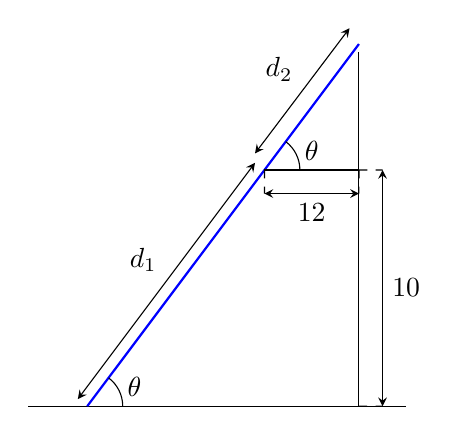
\begin{tikzpicture}[>=stealth, scale=0.3]
				\draw (0,0) -- (16,0) (14,0) -- (14,15);
				\coordinate (A) at (2.5,0); % Chân thang
				\coordinate (B) at (10,10); % Điểm chạm mái hiên
				\coordinate (C) at (14,15.33); % Ngọn thang chạm tường
				\coordinate (H) at (10,0); % Hình chiếu của B xuống đất
				\coordinate (K) at (14,10); % Hình chiếu của B vào tường
				\draw[thick, blue] (A) -- (C);
				% Vẽ mái hiên (đoạn nằm ngang)
				\draw (B) -- (K);
				% Kẻ đường gióng kích thước 10
				\draw[<->] (15,0) -- (15,10) node[midway, right] {$10$};
				\draw[dashed] (K) -- (15,10) (14,0) -- (15,0);
				% Kẻ đường gióng kích thước 12
				\draw[<->] (10,9) -- (14,9) node[midway, below] {$12$};
				\draw[dashed] (B) -- (10,9) (K) -- (14,9);
				\draw (4,0) arc (0:53:1.5);\node at (4.5,0.8) {$\theta$};
				\draw (11.5,10) arc (0:53:1.5);\node at (12,10.8) {$\theta$};
				\draw[<->] (2.1,0.3) -- (9.6,10.3) node[midway, above left] {$d_1$};
				\draw[<->] (9.6,10.7) -- (13.6,16) node[midway, above left] {$d_2$};
			\end{tikzpicture}
		}
		\noindent
		Ta có
		$$\begin{aligned}
			f'(\theta)=0 
			& \Leftrightarrow \dfrac{12\sin\theta}{\cos^2\theta}=\dfrac{10\cos\theta}{\sin^2\theta} \\
			& \Leftrightarrow \dfrac{\sin^3\theta}{\cos^3\theta}=\dfrac{10}{12} \\
			& \Leftrightarrow \tan^3\theta=\dfrac{5}{6} \\
			& \Leftrightarrow \tan\theta=\sqrt[3]{\dfrac{5}{6}} \\ 
			& \Leftrightarrow \theta=\theta_0\approx0{,}76 \, (\text{rad}).
		\end{aligned}$$
		Bảng biến thiên của $f(\theta)$
		\begin{center}
			
\begin{tikzpicture}[scale=1, >=stealth]
				\tkzTabInit[nocadre=false, lgt=1.2, espcl=2.5, deltacl=0.6]{$\theta$/1, $f'(\theta)$/0.6, $f(\theta)$/3}{$0$, $\theta_0$, $\dfrac{\pi}{2}$}
				\tkzTabLine{,-,0,+,}
				\tkzTabVar{+/, -/, +/}
			\end{tikzpicture}
		\end{center}
		Từ bảng biến thiên ta có $\min\limits_{\left(0;\dfrac{\pi}{2}\right)} f(\theta)=f\left(\theta_0\right)$ (m). \\
		Vậy độ dài ngắn nhất của chiếc thang cần thiết là $f\left(\theta_0\right)-\dfrac{1{,}2}{\sin\theta_0}\approx 29{,}3$ m.
	}
\end{ex}

\begin{ex}%[TT-ThieuHoa-ThanhHoa-L1-25-26]%[Vũ Nguyễn Hoàng Anh]%[0D0K2-5]
	Hai thí sinh $A$ và $B$ cùng tham gia một cuộc thi vấn đáp. Cán bộ coi thi đưa cho mỗi thí sinh một bộ câu hỏi gồm $10$ câu hỏi khác nhau, được đựng trong $10$ phong bì dán kín, có hình thức giống hệt nhau, mỗi phong bì đựng $1$ câu hỏi; thí sinh chọn $3$ phong bì để xác định câu hỏi của mình. Biết rằng bộ $10$ câu hỏi của các thí sinh là như nhau. Hai phong bì được gọi là giống nhau nếu chứa cùng một câu hỏi. Xác suất để $3$ phong bì $A$ chọn và $3$ phong bì $B$ chọn có ít nhất hai phong bì giống nhau là $\dfrac{a}{b}$ (trong đó $\dfrac{a}{b}$ là phân số tối giản và $a,b\in\mathbb{N}$). Tính $a^2+b^2$.
	
	\shortans{3721}
	\loigiai{
		Số cách để $A$ và $B$ chọn đúng hai phong bì giống nhau ($A$ và $B$ chọn $2$ phong bì giống nhau rồi  $A$ và $B$ lần lượt chọn $1$ phong bì khác với hai cái vừa chọn và khác nhau) là $\mathrm{C}^2_{10}\cdot \mathrm{C}^1_8\cdot \mathrm{C}^1_7$.\\
		Số cách để $A$ và $B$ chọn được ba phong bì giống nhau là $\mathrm{C}^3_{10}$.\\
		Suy ra xác suất cần tìm là $\dfrac{\mathrm{C}^2_{10}\cdot \mathrm{C}^1_8\cdot \mathrm{C}^1_7+\mathrm{C}^3_{10}}{\mathrm{C}^3_{10}\mathrm{C}^3_{10}}=\dfrac{11}{60}$.\\
		Do dó $a=11$, $b=60$ và $a^2+b^2=3\,721$.
	}
\end{ex}

\begin{ex}%[TT-ThieuHoa-ThanhHoa-L1-25-26]%[Vũ Nguyễn Hoàng Anh]%[1H8K7-6]
	\immini[thm]{
		Bác Bình có một chậu cảnh trồng hoa hình chóp cụt tứ giác đều với chiều cao $30$ cm, cạnh đáy lần lượt là $20$ cm và $40$ cm.
	Bác Bình đổ đất vào chậu để tiến hành trồng, chiều cao của đất bằng $ \dfrac{2}{3} $ chiều cao của chậu. Tính thể tích lượng đất bác Bình đã đổ vào chậu theo dm$^3$ (làm tròn kết quả đến hàng phần mười). 
	}{
		\begin{tikzpicture}[line cap=round, line join=round,font=\footnotesize,>=stealth, scale=0.7]
			\tikzset{label style/.style={font=\footnotesize}}
			\clip (-0.5,-2) rectangle (5.5,1.8);
			\def\a{4}
			\def\h{4.5}
			\path 	(0:0) coordinate (A)
			++(0:\a) coordinate (D)
			++(50:\a/2) coordinate (C)
			($(A)+(C)-(D)$) coordinate (B)
			(intersection of A--C and B--D) coordinate (O)
			($(O)-(90:\h)$) coordinate (S);
			\foreach\x in {A,B,C,D}{
				\path ($(S)!0.5!(\x)$) coordinate (\x')
				($(\x)!1/3!(\x')$) coordinate (\x1);}
			\path (intersection of C1--B1 and C--D) coordinate (a)
			(intersection of A1--B1 and A--D) coordinate (b); 
			\fill[brown!30] (A1)--(B1)--(C1)--(D1)
			(A')--(A1)--(D1)--(D')
			(D')--(C')--(C1)--(D1);
			\draw (a)--(B1)--(b);
			\draw (A')--(D')--(C')
			(A)--(D)--(C)--(B)--(A)--(A') (C)--(C') (D)--(D') (A1)--(D1)--(C1) (B1)--(B);
			\draw[dashed] (C')--(B')--(A') (C1)--(a) (b)--(A1) (B')--(B1);
		\end{tikzpicture}
	}
	\shortans{14,5}
	\loigiai{
		Phần đất trong chậu cũng tạo thành một khối chóp cụt đều có chiều cao là $\dfrac{2}{3}\cdot 30=20$ cm và có một đáy có cạnh là $20$ cm, một đáy có cạnh là $\dfrac{20+2\cdot 40}{3}=\dfrac{100}{3}$ cm. Do đó thể tích khối đất đã đổ vào là
		\[ \frac{1}{3}\cdot 20\left[20^2+\left(\frac{100}{2}\right)^2+20\cdot \frac{100}{3}\right]=\frac{392\,000}{27}\text{ cm}^3\approx 14{,}5\text{ dm}^3. \] 
	}
\end{ex}


\Closesolutionfile{ans}

% \indapan{4}{ans/ans-TT-ThieuHoa-ThanhHoa-L1-25-26}


=======
\begin{name}
	{\tenchude}
	{THPT Thiệu Hóa, Thanh Hóa}
	{LỚP TOÁN THẦY PHÁT}
	{ Với một người luôn biết cố gắng, không có gì là không thể}
\end{name}

\TN
\setcounter{ex}{0}
\Opensolutionfile{ans}[ans/ans-TT-ThieuHoa-ThanhHoa-L1-25-26]
%Câu 1
\begin{ex}%[Duong Xuan Loi]%[1H8N4-3]
	Cho hình chóp $S.ABC$ có $SA\perp(ABC)$ và $AB\perp BC$. Góc giữa hai mặt phẳng $(SBC)$ và $(ABC)$ là góc nào sau đây?		
	\choice
	{$\widehat{SIA}$ với $I$ là trung điểm của $BC$}
	{\True $\widehat{SBA}$}
	{$\widehat{SCB}$}
	{$\widehat{SCA}$}
	\loigiai{
		\immini{
			Ta có $\heva{&(SBC) \cap (ABC) = BC \\ &AB \subset (ABC), SB \subset (SBC) .}$\\
			Mặt khác
			\begin{itemize}
				\item $AB \perp BC$ (giả thiết).
				\item $SA \perp (ABC) \Rightarrow SA \perp BC$.
			\end{itemize}
			Suy ra $BC \perp (SAB) \Rightarrow BC \perp SB$.\\
			Vậy $\left((SBC),(ABC)\right)=(SB,AB)=\widehat{SBA}$ (vì $\triangle SAB$ vuông tại $A$).
		}{
			\begin{tikzpicture}[scale=0.8, font=\footnotesize, line join=round, line cap=round,>=stealth]
				\path
				(0,0) coordinate (A)
				(1.5,-1.2) coordinate (B)
				(4,0) coordinate (C)
				($(A)+(0,3.0)$) coordinate (S)	
				;
				\draw (S)--(A)--(B)--(C)--cycle (S)--(B);	
				\draw[dashed] (A)--(C);	
				\foreach \p/\q in {S/90,A/180,B/-90,C/0}
				\fill[black] (\p) circle (1.0pt) ($(\p)+(\q:3mm)$) node{$\p$};
				\draw pic[draw, angle radius=2mm] {right angle = S--A--B};
				\draw pic[draw, angle radius=2mm] {right angle = A--B--C};
			\end{tikzpicture}
		}
	}
\end{ex}
\begin{ex}%[Duong Xuan Loi]%[2H2N1-1]
	Cho hình lăng trụ $ABC.A'B'C'$, $M$ là trung điểm của $BB'$. Đặt $\overrightarrow{CA}=\overrightarrow{a}$, $\overrightarrow{CB}=\overrightarrow{b}$, $\overrightarrow{AA'}=\overrightarrow{c}$. Khẳng định nào sau đây đúng?
	\choice
	{\True $\overrightarrow{AM}=\overrightarrow{b}-\overrightarrow{a}+\dfrac{1}{2}\overrightarrow{c}$}
	{$\overrightarrow{AM}=\overrightarrow{a}+\overrightarrow{c}-\dfrac{1}{2}\overrightarrow{b}$}
	{$\overrightarrow{AM}=\overrightarrow{b}+\overrightarrow{c}-\dfrac{1}{2}\overrightarrow{a}$}
	{$\overrightarrow{AM}=\overrightarrow{a}-\overrightarrow{c}+\dfrac{1}{2}\overrightarrow{b}$}
	\loigiai{
		\immini{
			Ta có $\overrightarrow{AM} = \overrightarrow{AB} + \overrightarrow{BM} = \left( \overrightarrow{CB} - \overrightarrow{CA} \right) + \dfrac{1}{2}\overrightarrow{BB'}$.\\
			Mặt khác $\overrightarrow{BB'} = \overrightarrow{AA'}$.\\
			Suy ra $\overrightarrow{AM} = \overrightarrow{b} - \overrightarrow{a} + \dfrac{1}{2}\overrightarrow{c}$.
		}{
			\begin{tikzpicture}[scale=0.7, font=\footnotesize, line join=round, line cap=round,>=stealth]
				\path
				(0,0)coordinate (A)
				(1.1,-1.5)coordinate (B)
				(4,-0.5)coordinate (C)
				($(A)+(0,3.8)$) coordinate (A')
				($(A')+(B)-(A)$)coordinate (B')
				($(A')+(C)-(A)$)coordinate (C')		
				($(B')!0.5!(B)$) coordinate (M)					
				;
				\draw (A)--(B)--(C)--(C')--(B')--(A')--cycle (A')--(C') (B)--(B') (A)--(M);
				\draw[dashed] (A)--(C);	
				\foreach \p/\q in {A/180,B/-90,C/0,A'/180,B'/70,C'/0,M/0}
				\fill[black] (\p) circle (1.0pt)node[shift={(\q:3mm)}]{$\p$};
			\end{tikzpicture}
	}}
\end{ex}

\begin{ex}%[Duong Xuan Loi]%[1D6N4-2]
	Tích các nghiệm của phương trình $2^{x^2-2x}=8$ là
	\choice
	{$2$}
	{$0$}
	{$3$}
	{\True $-3$}
	\loigiai{
		Ta có \[2^{x^2-2x}=8\Leftrightarrow 2^{x^2-2x}=2^3\Leftrightarrow x^2-2x=3\Leftrightarrow x^2-2x-3=0\Leftrightarrow \hoac{& x= -1\\ & x=3.}\]
		Tích các nghiệm của phương trình là $(-1)\cdot3=-3$.
	}
\end{ex}

\begin{ex}%[Duong Xuan Loi]%[2D1N2-1]
	Cho hàm số $f(x)$ có đạo hàm $f'(x)=(x+1)x^2(x-3)^3$, $\forall x\in\mathbb{R}$. Hàm số đã cho có bao nhiêu điểm cực trị?
	\choice
	{$3$}
	{\True $2$}
	{$5$}
	{$1$}
	\loigiai{
		Ta có $f'(x)=0\Leftrightarrow\hoac{&x=-1 \text{ (nghiệm bội lẻ)}\\& x=0 \text{ (nghiệm bội chẵn)}\\ & x=3 \text{ (nghiệm bội lẻ)}.}$\\
		Bảng xét dấu
		\begin{center}
			\begin{tikzpicture}
				\tkzTabInit[nocadre=false,lgt=1.2,espcl=2.5,deltacl=0.6]
				{$x$ /0.6, $f'(x)$ /0.6, $f(x)$ /2.5}
				{$-\infty$,$-1$,$0$,$3$,$+\infty$}
				\tkzTabLine{,+,$0$,-,$0$,-,$0$,+,}
				\tkzTabVar{-/,+/CĐ,R,-/CT,+/$+\infty$}
			\end{tikzpicture}
		\end{center}
		Từ bảng xét dấu suy ra hàm số có $2$ cực trị.		
	}
\end{ex}

\begin{ex}%[Thi thử, THPT Thiệu Hóa, Thanh Hóa, 2026]%[Thành Đức Trung]%[1D3V2-7]
	Cho hai đồ thị $y = \dfrac{1}{x}$ và $y = \sqrt{x}$ cắt nhau tại điểm $A(1;1)$. Với số thực $t>1$, đường thẳng $y=t$ lần lượt cắt đồ thị $y = \dfrac{1}{x}$ và $y=  \sqrt{x}$ tại các điểm $B$ và $C$.
	\begin{center}
		\begin{tikzpicture}[scale=1.3, font=\normalsize, >=stealth]  
			\draw[->] (-1,0)--(0,0) node[below left]{$O$}--(7,0) node[below]{$x$};
			\draw[->] (0,-1) --(0,3.5) node[right]{$y$};
			\draw [black,thick, domain=0:5.5, samples=100] plot(\x,{sqrt((\x))}) node[above]{$y = \sqrt{x}$};
			\draw [black,thick, domain=0.35:5, samples=100] plot(\x,{1/(\x)}) node[right]{$y = \tfrac{1}{x}$};
			\draw[fill = black] (0,0) circle (1pt);
			\draw (-1,2)--(6,2) node[below] {$y=t$} (4,-1)--(4,3);
			\path 
			(1,1) coordinate (A)
			(.5,2) coordinate (B)
			(4,2) coordinate (C)
			(4,.25) coordinate (D)
			;
			\draw[dashed] (1,0) node[below]{$1$} -- (A) -- (0,1) node[left]{$1$};
			\draw (A)--(B)--(C)--(A)--(D)--(C);
			\fill[color=blue,opacity=.2] (A)--(B)--(C)--(A);
			\fill[color=red,opacity=.2] (A)--(D)--(C)--(A);
			\foreach \x/\g in{A/80, B/60, C/-45, D/45}
			\fill[black](\x)circle(1pt)($(\x)+(\g:2.5mm)$)node{$\x$};
		\end{tikzpicture}
	\end{center}
	Từ $C$ kẻ đường thẳng song song với trục $Oy$, cắt đồ thị $y = \dfrac{1}{x}$ tại điểm $D$. Gọi $f(t)$ là diện tích tam giác $ACB$ và $g(t)$ là diện tích tam giác $ADC$. Tính $L = \displaystyle\lim_{t\to1^+}\dfrac{g(t)}{f(t)}$.
	\choice
	{$L = +\infty$}
	{$L = \dfrac{5}{3}$}
	{$L = 0$}
	{\True $L = 2$}
	\loigiai
	{
		Vì $B$ là giao điểm của hai đồ thị hàm số $y=t$ và $y=\dfrac{1}{x}$ nên $B\left(\dfrac{1}{t};t\right)$. \\
		Vì $C$ là giao điểm của hai đồ thị hàm số $y=t$ và $y=\sqrt{x}$ nên $C\left(t^2;t\right)$. \\
		Đường thẳng đi qua $C$ và song song với $Oy$ có phương trình là $x=t^2$. \\
		Vì $D$ là giao điểm của hai đồ thị hàm số $y=\dfrac{1}{x}$ và $x=t^2$ nên $D\left(t^2;\dfrac{1}{t^2}\right)$. \\
		Xét $\triangle ABC$ có
		\[f(t) = S_{\triangle ABC} = \dfrac{1}{2}BC\cdot\mathrm{d}\left(A,BC\right) = \dfrac{1}{2}\cdot \left(t^2-\dfrac{1}{t}\right)\cdot \left(t - 1\right) = \dfrac{\left(t^3-1\right)(t-1)}{2t}.\]
		Xét $\triangle ADC$ có
		\[g(t) = S_{\triangle ADC} = \dfrac{1}{2}CD\cdot\mathrm{d}\left(A,CD\right) = \dfrac{1}{2}\cdot \left(t - \dfrac{1}{t^2}\right)\cdot \left(t^2 - 1\right) = \dfrac{\left(t^3-1\right)\left(t^2-1\right)}{2t^2}.\]
		Suy ra $L = \displaystyle\lim_{t\to1^+}\dfrac{g(t)}{f(t)} = \displaystyle\lim_{t\to1^+} \dfrac{t^2-1}{t(t-1)} = 2$.
	}
\end{ex}

%%%% Câu 6
\begin{ex}%[Thi thử, THPT Thiệu Hóa, Thanh Hóa, 2026]%[Thành Đức Trung]%[0D1N2-2] 
	Số tập con của tập hợp gồm $2\,026$ phần tử là
	\choice
	{$2 \times 2026$}
	{$2026$}
	{$2026^2$}
	{\True $2^{2026}$}
	\loigiai
	{
		Số tập con của một tập hợp có $n$ phần tử là $2^n$. \\
		Với $n = 2\,026$, số tập con của tập hợp đã cho là $2^{2\,026}$.
	}
\end{ex}

%%%% Câu 7
\begin{ex}%[Thi thử, THPT Thiệu Hóa, Thanh Hóa, 2026]%[Thành Đức Trung]%[2H2V2-2]
	Trong không gian $Oxyz$, cho hai điểm $A(1;2;1)$, $B(2;-1;3)$ và điểm $M(a;b;0)$ sao cho $MA^2 + MB^2$ nhỏ nhất. Giá trị của $a+b$ là
	\choice
	{$3$}
	{$-2$}
	{$1$}
	{\True $2$}
	\loigiai
	{
		Gọi $I$ là trung điểm của đoạn thẳng $AB$ suy ra $I\left( \dfrac{3}{2}; \dfrac{1}{2}; 2 \right)$.\\
		Khi đó $MA^2 + MB^2 = \left(\overrightarrow{MI} + \overrightarrow{IA}\right)^2 + \left(\overrightarrow{MI} + \overrightarrow{IB}\right)^2 = 2MI^2 + IA^2 + IB^2$ (do $\overrightarrow{IA} + \overrightarrow{IB} = \overrightarrow{0}$).\\
		Để $MA^2 + MB^2$ nhỏ nhất thì $MI$ nhỏ nhất. Mà $M(a;b;0) \in (Oxy)$, do đó $M$ là hình chiếu vuông góc của $I$ trên mặt phẳng $(Oxy)$.\\
		Suy ra $M\left( \dfrac{3}{2}; \dfrac{1}{2}; 0 \right)$, tức là $a = \dfrac{3}{2}$ và $b = \dfrac{1}{2}$.\\
		Vậy $a + b = \dfrac{3}{2} + \dfrac{1}{2} = 2$.
	}
\end{ex}

%%%% Câu 8
\begin{ex}%[Thi thử, THPT Thiệu Hóa, Thanh Hóa, 2026]%[Thành Đức Trung]%[2H2N2-2]
	Trong không gian với hệ tọa độ $Oxyz$, cho hai điểm $A(-3;4;5)$, $B(-1;0;1)$. Tìm tọa độ điểm $M$ thỏa mãn $\overrightarrow{MA} + \overrightarrow{MB} = \overrightarrow{0}$.
	\choice
	{$M(-4;-4;-4)$}
	{$M(4;4;4)$}
	{\True $M(-2;2;3)$}
	{$M(1;2;3)$}
	\loigiai
	{
		Điều kiện $\overrightarrow{MA} + \overrightarrow{MB} = \overrightarrow{0}$ tương đương với $M$ là trung điểm của đoạn thẳng $AB$.\\
		Tọa độ điểm $M$ là
		$\heva{&x_M = \dfrac{x_A + x_B}{2} = \dfrac{-3 + (-1)}{2} = -2 \\ &y_M = \dfrac{y_A + y_B}{2} = \dfrac{4 + 0}{2} = 2 \\ &z_M = \dfrac{z_A + z_B}{2} = \dfrac{5 + 1}{2} = 3.}$\\
		Vậy $M(-2;2;3)$.
	}
\end{ex}


\begin{ex}%[TT-ThieuHoa-ThanhHoa-L1-25-26]%[Vũ Nguyễn Hoàng Anh]%[1D2H3-4]
	Diện tích rừng tự nhiên của nước ta năm $2\,021$ là xấp xỉ $10\,171\,757$ ha. 
	Giả sử tỉ lệ tăng diện tích rừng tự nhiên hằng năm kể từ năm $2\,021$ là $0{,}7\%$/năm. 
	Diện tích rừng tự nhiên của nước ta vào năm $2\,025$ xấp xỉ bằng
	\choice
	{$10\,468\,251$ ha}
	{\True $10\,459\,571$ ha}
	{$10\,386\,863$ ha}
	{$10\,532\,788$ ha}
	\loigiai{
		 Diện tích rừng của nước ta vào năm $2\,025$ xấp xỉ $10\,171\,757(1+0{,}7\%)^4\approx 10\,459\,571$ ha.
	}
\end{ex}

\begin{ex}%[TT-ThieuHoa-ThanhHoa-L1-25-26]%[Vũ Nguyễn Hoàng Anh]%[2D1N1-2]
	\immini{
		Cho hàm số $y=f(x)$ có đồ thị như hình vẽ.  
	Hãy chọn đáp án đúng.
	\choice
	{Hàm số nghịch biến trên $(0;2)$}
	{Hàm số đồng biến trên $(-\infty;0)$ và $(2;+\infty)$}
	{Hàm số đồng biến trên $(-1;0)$ và $(2;3)$}
	{\True Hàm số nghịch biến trên $(-\infty;0)$ và $(2;+\infty)$}
	}{
		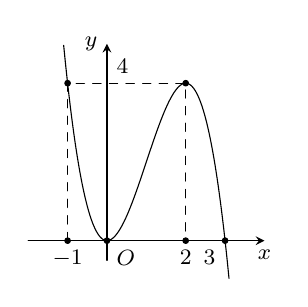
\begin{tikzpicture}[line cap=round, line join=round,font=\footnotesize,>=stealth, scale=0.5]
			\tikzset{label style/.style={font=\footnotesize}}
			\draw[->] (-2,0)--(4,0)node[below]{$x$};
			\draw[->] (0,-0.5)--(0,5) node[left]{$y$};
			\draw[dashed] (-1,0)node[below]{$-1$}--(-1,4)--(0,4) node[above right]{$4$}--(2,4)--(2,0) node[below]{$2$};
			\draw[fill=black] (0,0) circle (2pt) node[below right]{$O$}
			(3,0) circle (2 pt) node[below left]{$3$}
			(-1,0) circle (2pt)
			(2,0) circle (2pt)
			(-1,4) circle (2pt)
			(2,4) circle (2pt);
			\draw[smooth, samples=100] plot[domain=-1.1:3.1] (\x, { -(\x)^2*(\x-3) });
			
		\end{tikzpicture}
	}
	\loigiai{
		Dựa vào đồ thị hàm số, hàm số nghịch biến trên các khoảng $(-\infty;0)$ và $(2;+\infty)$.  
	}
\end{ex}

\begin{ex}%[TT-ThieuHoa-ThanhHoa-L1-25-26]%[Vũ Nguyễn Hoàng Anh]%[2H2H2-2] 
	Trong không gian với hệ trục tọa độ cho trước (đơn vị đo lấy theo kilmet), 
	ra đa phát hiện một máy bay di chuyển với vận tốc và hướng không đổi 
	từ điểm $A(750;450;7)$ đến điểm $B(950;550;9)$ trong $10$ phút.  
	Nếu máy bay tiếp tục giữ nguyên vận tốc và hướng bay trong $10$ phút nữa 
	đến điểm $C(x;y;z)$ thì $x+y+z$ bằng
	\choice
	{$1\,931$}
	{\True $1\,811$}
	{$1\,691$}
	{$1\,781$}
	\loigiai{
		Từ giả thiết, ta thấy $B$ là trung điểm $AC$, do đó $C=(1\,150;650;11)$. Từ đó $x+y+z= 1\,811$.
	}
\end{ex}

\begin{ex}%[TT-ThieuHoa-ThanhHoa-L1-25-26]%[Vũ Nguyễn Hoàng Anh]%[2D4N1-3] 
	Thời gian (phút) truy cập Internet mỗi buổi tối của một số học sinh được cho trong bảng sau
	\begin{center}
		\begin{tabular}{|c|c|c|c|c|c|}
			\hline
			Thời gian (phút) & $[9{,}5;12{,}5)$ & $[12{,}5;15{,}5)$ & $[15{,}5;18{,}5)$ & $[18{,}5;21{,}5)$ & $[21{,}5;24{,}5)$ \\
			\hline
			Số học sinh & $3$ & $12$ & $15$ & $24$ & $2$ \\
			\hline
		\end{tabular}
	\end{center}
	Khoảng tứ phân vị của mẫu số liệu ghép nhóm là
	\choice
	{$4{,}63$}
	{$10{,}75$}
	{$4{,}38$}
	{\True $4{,}75$}
	\loigiai{
		Ta có bảng
		\begin{center}
			\begin{tabular}{|c|c|c|c|c|c|}
				\hline
				Thời gian (phút) & $[9{,}5;12{,}5)$ & $[12{,}5;15{,}5)$ & $[15{,}5;18{,}5)$ & $[18{,}5;21{,}5)$ & $[21{,}5;24{,}5)$ \\
				\hline
				Số học sinh & $3$ & $12$ & $15$ & $24$ & $2$ \\
				\hline
				Tần số tích lũy & $3$ &$15$ & $30$ &$54$&$56$\\
				\hline 
			\end{tabular}
		\end{center}
		Suy ra $Q_1=12{,}5+\dfrac{3\left(\dfrac{56}{4}-3\right)}{12}=15{,}25$, $Q_3=18{,}5+\dfrac{3\left(\dfrac{3\cdot 56}{4}-30\right)}{24}=20$. Vậy khoảng tứ phân vị của mẫu số liệu là $\Delta Q=Q_3-Q_1=4{,}75$.	}
\end{ex}


\cauds

\begin{ex}%[Duong Xuan Loi]%[2D1H5-3]
	Cho hàm số $y=f(x)$ có bảng biến thiên như sau
	\begin{center}
		
\begin{tikzpicture}
			\tkzTabInit[nocadre=false,lgt=1.2,espcl=2.5,deltacl=0.6]
			{$x$ /0.6, $f'(x)$ /0.6, $f(x)$ /2.5}
			{$-\infty$,$-1$,$1$,$+\infty$}
			\tkzTabLine{,+,$0$,-,$0$,+,}
			\tkzTabVar{-/$-\infty$,+/$3$,-/$-1$,+/$+\infty$}
		\end{tikzpicture}
	\end{center}
	Các mệnh đề sau đúng hay sai?
	\choiceTF
	{\True $f'(x)=0\Leftrightarrow\hoac{&x=-1\\&x=1}$}
	{\True Đồ thị hàm số $y=f(x)$ cắt trục $Ox$ tại $3$ điểm phân biệt}
	{Giá trị cực tiểu của hàm số bằng $1$}
	{\True Hàm số $y=f(2-x)$ đồng biến trên $(1;3)$}
	\loigiai{
		\begin{itemchoice}
			\itemch Ta có $f'(x)=0\Leftrightarrow\hoac{&x=-1\\&x=1.}$		
			\itemch Ta có $y_{\text{CĐ}}\cdot y_{\text{CT}}=3\cdot(-1)=-3<0$ suy ra đồ thị hàm số $y=f(x)$ cắt trục $Ox$ tại $3$ điểm phân biệt.
			\itemch Ta có $y_{\text{CT}}=-1$.
			\itemch Xét hàm số $y=f(2-x)$.\\
			Có $y'=-f'(2-x)$.\\
			$y'=0\Leftrightarrow f'(2-x)=0\Leftrightarrow \hoac{& 2-x=-1 \\ & 2-x=1}\Leftrightarrow\hoac{& x=3 \\ & x=1.}$\\
			Bảng xét dấu
			\begin{center}
				
\begin{tikzpicture}
					\tkzTabInit[nocadre=false,lgt=1.2,espcl=2.5,deltacl=0.6]
					{$x$ /0.6, $y'$ /0.6, $y$ /2.5}
					{$-\infty$,$1$,$3$,$+\infty$}
					\tkzTabLine{,-,$0$,+,$0$,-,}
					\tkzTabVar{+/,-/,+/,-/}
				\end{tikzpicture}
			\end{center}
			Từ bảng xét dấu suy ra hàm số đồng biến trên $(1;3)$.
		\end{itemchoice}
	}
\end{ex}

\begin{ex}%[Thi thử, THPT Thiệu Hóa, Thanh Hóa, 2026]%[Thành Đức Trung]%[2D3H2-3]
	Thời gian hoàn thành một bài viết chính tả của một số học sinh lớp $4$ hai trường X và Y được ghi lại ở bảng sau
	\begin{center}
		\begin{tabular}{|c|c|c|c|c|c|}
			\hline
			Thời gian (phút)	& $\left[ 6;7 \right)$ & $\left[ 7;8 \right)$ & $\left[ 8;9 \right)$ & $\left[ 9;10 \right)$ & $\left[ 10;11 \right)$ \\
			\hline
			Số học sinh trường X	& $8$ & $10$ & $13$ & $10$ & $9$ \\
			\hline
			Số học sinh trường Y	& $4$ & $12$ & $17$ & $14$ & $3$ \\
			\hline
		\end{tabular}
	\end{center}
	\choiceTF
	{\True Nếu so sánh theo độ lệch chuẩn thì học sinh trường Y có tốc độ viết đồng đều hơn}
	{Nếu so sánh theo khoảng tứ phân vị thì học sinh trường X có tốc độ viết đồng đều hơn}
	{Phương sai của mẫu số liệu ghép nhóm của trường X là $1{,}08$ và phương sai của mẫu số liệu ghép nhóm của trường Y là $1{,}7584$}
	{\True Nếu so sánh theo số trung bình thì học sinh trường Y viết nhanh hơn}
	\loigiai
	{
		Với trường X, tổng số học sinh
		\[
		n_X = 8+10+13+10+9 = 50.
		\]
		\begin{itemize}
			
			\item {Số trung bình}
			\[
			\overline{x}_X
			= \dfrac{8\cdot6{,}5 + 10\cdot7{,}5 + 13\cdot8{,}5 + 10\cdot9{,}5 + 9\cdot10{,}5}{50}
			= 8{,}54\ (\text{phút}).
			\]
			\item {Khoảng tứ phân vị}
			\[
			Q_{1X} = 7 + \dfrac{12{,}5 - 8}{10}\cdot 1 = 7{,}45.
			\]
			\[
			Q_{3X} = 9 + \dfrac{37{,}5 - 31}{10}\cdot 1 = 9{,}65.
			\]
			\[
			\Delta Q_X = 2{,}2.
			\]
			
			\item {Phương sai và độ lệch chuẩn}
			\[
			s_X^2 = \dfrac{1}{50}\sum n_i(x_i-\overline{x}_X)^2 = 1{,}7584,
			\qquad
			s_X =\sqrt{1{,}7854} = 1{,}33.
			\]
			
		\end{itemize}
		Với trường Y, tổng số học sinh
		\[
		n_Y = 4+12+17+14+3 = 50.
		\]
		\begin{itemize}
			\item {Số trung bình}
			
			\[
			\overline{x}_Y
			= \dfrac{4\cdot6{,}5 + 12\cdot7{,}5 + 17\cdot8{,}5 + 14\cdot9{,}5 + 3\cdot10{,}5}{50}
			= 8{,}50\ (\text{phút}).
			\]
			
			\item {Khoảng tứ phân vị}
			\[
			Q_{1Y} = 7 + \dfrac{12{,}5 - 4}{12}\cdot 1 \approx 7{,}71.
			\]			
			\[
			Q_{3Y} = 9 + \dfrac{37{,}5 - 33}{14}\cdot 1 \approx 9{,}32.
			\]
			\[
			\Delta Q_Y \approx 1{,}61.
			\]
			\item {Phương sai và độ lệch chuẩn}
			
			\[
			s_Y^2 = \dfrac{1}{50}\sum n_i(x_i-\overline{x}_Y)^2 \approx 1{,}08,
			\qquad
			s_Y \approx \sqrt{1{,}08} = 1{,}03.
			\]
			
		\end{itemize}
	}
\end{ex}

%%%% Câu 15
\begin{ex}%[Thi thử, THPT Thiệu Hóa, Thanh Hóa, 2026]%[Thành Đức Trung]%[1H8C7-9]
	\immini{Kim tự tháp Cheops là kim tự tháp lớn nhất trong các kim tự tháp ở Ai Cập, được xây dựng vào thế kỉ thứ $26$ trước Công nguyên và là một trong bảy kì quan của thế giới cổ đại. Kim tự tháp có dạng hình chóp $S.ABCD$ với đáy là hình vuông $ABCD$ tâm $H$ và cạnh đáy dài $262\,$m, các cạnh bên bằng nhau và dài $230\,$m (kích thước hiện nay).}{	
		\begin{tikzpicture}[line join = round,scale=0.7,xscale=0.7,yscale=1.2]
			\definecolor{vang}{HTML}{f2e6bc}
			\path (-3, 0.2) coordinate (A) -- (0, 0) coordinate (B) -- (2, 4) coordinate (C)
			(8, 0.1) coordinate (D);
			\path[inner color=vang,outer color=vang!60!white] (A)--(B)--(C)--cycle;
			\path[inner color=vang,outer color=vang!60!white] (D)--(B)--(C)--cycle;
			\foreach \i in {1,...,18}{
				\pgfmathsetmacro{\tiso}{\i/19}
				\draw[vang!65!orange,opacity=0.65] ($(B)!\tiso!(C)$)--($(B)!\tiso!(A)$);
				\draw[vang!65!orange,opacity=0.65]($(A)!\tiso!(C)$)--($(A)!\tiso!(B)$);
				\draw[vang!65!orange,opacity=0.65] ($(B)!\tiso!(C)$)--($(B)!\tiso!(D)$);
				\draw[vang!65!orange,opacity=0.65]($(D)!\tiso!(C)$)--($(D)!\tiso!(B)$);
			}
			\draw[black!65!gray] (B)--(D)--(C) (A)--(B)--(C)--cycle;
		\end{tikzpicture}
	}
	\noindent Biết căn phòng chứa đựng thông tin khảo cổ có dạng hình lập phương với thể tích $64\,$m$^3$ ngay tại trung tâm, có cạnh đáy song song với cạnh đáy của kim tự tháp và $H$ cũng là tâm của mặt sàn căn phòng. Các nhà khảo cổ muốn tạo một lỗ khoan từ bên ngoài vào căn phòng này.
	\choiceTF
	{\True Kim tự tháp có hình dạng là một hình chóp đều}
	{Chiều cao của kim tự tháp là $\sqrt{18\,579}\,$m}
	{\True Phần không gian mà kim tự tháp chiếm chỗ là $3\,118\,752\,$m$^3$ \textit{(làm tròn kết quả đến hàng đơn vị)}}
	{\True Chiều dài nhỏ nhất của lỗ khoan mà các nhà khảo cổ muốn tạo bằng $90$ mét \textit{(làm tròn kết quả đến hàng đơn vị)}}
	\loigiai
	{
		\begin{center}
			\begin{tikzpicture}[scale=0.9, font=\footnotesize, line join=round, line cap=round, >=stealth]
				\coordinate (A) at (2,2.5);
				\coordinate (B) at (0,0);
				\coordinate (C) at (6,0);
				\coordinate (D) at ($(A)+(C)-(B)$);
				\coordinate (H) at ($(A)!0.5!(C)$); % Giả sử H là hình chiếu của S
				\coordinate (S) at ($(H)+(0,5.5)$);
				\coordinate (M) at ($(C)!0.5!(D)$);
				\coordinate (F) at ($(S)!0.68!(M)$);
				\coordinate (A2) at ($(A)!0.65!(H)$); 
				\coordinate (B2) at ($(B)!0.65!(H)$);
				\coordinate (C2) at ($(C)!0.65!(H)$);
				\coordinate (D2) at ($(D)!0.65!(H)$);
				\coordinate (A1) at ($(A2)+(0,1.3)$);
				\coordinate (B1) at ($(B2)+(0,1.3)$);
				\coordinate (C1) at ($(C2)+(0,1.3)$);
				\coordinate (D1) at ($(D2)+(0,1.3)$);
				\coordinate (I) at ($(C1)!0.5!(D1)$);
				\draw[dashed] (S)--(A) (A)--(B) (A)--(D) (B)--(D) (A)--(C) (S)--(H) (H)--(M) (I)--(F);
				\draw (M)--(S)--(B) (S)--(C) (S)--(D) (B)--(C) (C)--(D);
				\draw[red, dashed, thick] (A1)--(B1)--(C1)--(D1)--cycle;
				\draw[red, dashed, thick] (A2)--(B2)--(C2)--(D2)--cycle;
				\draw[red, dashed, thick] (A1)--(A2) (B1)--(B2) (C1)--(C2) (D1)--(D2);
				\foreach \p/\pos in {S/above, A/left, B/left, C/right, D/right, H/below, M/below right, F/right, I/left}
				\fill[black] (\p) circle (1.5pt) node[\pos] {$\p$};
			\end{tikzpicture}\hspace*{1cm}
			\begin{tikzpicture}[>=stealth, scale=0.8, font=\footnotesize]
				\coordinate (S) at (0,6);
				\coordinate (H) at (0,0);
				\coordinate (M) at (4,0);
				\coordinate (N) at (1,0);
				\coordinate (I) at (1,1.5);
				\path ($(S)!(I)!(M)$) coordinate (F);
				\draw[dashed] (I)--(N);
				\draw (S)--(M) (I)--(F);
				\draw[->] (H)--($(S)+(0,0.5)$) node[left]{$y$};
				\draw[->] (H)--($(M)+(0.5,0)$) node[below]{$x$};
				\foreach\x/\y in {H/-135,N/-90,S/180,I/135,M/-90,F/40} \draw[fill=black] (\x) circle (1.2pt)+(\y:0.3) node{$\x$};
			\end{tikzpicture}
		\end{center}
		\begin{itemchoice}
			\itemch Vì đáy $ABCD$ là hình vuông và các cạnh bên bằng nhau nên $S.ABCD$ là hình chóp tứ giác đều.
			\itemch Ta có nửa đường chéo đáy là $AH = \dfrac{AC}{2} = \dfrac{262\sqrt{2}}{2} = 131\sqrt{2}\,$m. \\
			Chiều cao kim tự tháp là $h=SH = \sqrt{SA^2 - AH^2} = \sqrt{230^2 - \left(131\sqrt{2}\right)^2} = \sqrt{18\,578}\,$m.
			\itemch Thể tích kim tự tháp là $V = \dfrac{1}{3} \cdot S_{ABCD} \cdot SH = \dfrac{1}{3} \cdot 262^2 \cdot \sqrt{18\,578} \approx 3\,118\,752\,$m$^3$ (làm tròn đến hàng đơn vị).
			\itemch Để mũi khoan có chiều dài ngắn nhất, ta cần khoan từ mặt bên vào vị trí cạnh của khối lập phương. Khoảng cách ngắn nhất là khoảng cách từ một điểm $I$ thuộc cạnh trên của khối lập phương đến mặt bên của hình chóp.\\
			Gọi $M$ là trung điểm của cạnh $CD$, thì $HM=131$ m. Dựng hệ trục tọa độ $Oxy$ sao cho $H(0;0)$, $M(131;0)$, $S\left(0;h\right)$. Đường thẳng $SM$ có phương trình $\dfrac{x}{131}+\dfrac{y}{h}=1$.\\
			Do căn phòng có thể tích $64$ m$^3$ nên độ dài cạnh của phòng là $IN=4$ m. Suy ra $I(2;4)$. Vậy độ dài lỗ khoan nhỏ nhất là
			\[ \mathrm{d}(I,SM)=\dfrac{\left| \dfrac{2}{131}+\dfrac{4}{h}-1 \right|}{\sqrt{\dfrac{1}{131^2}+\dfrac{1}{h^2}}}\approx 90\text{ m}. \]
		\end{itemchoice}
	}
\end{ex}

\begin{ex}%[TT-ThieuHoa-ThanhHoa-L1-25-26]%[Vũ Nguyễn Hoàng Anh]%[2H2K2-6] 
	\immini{
		Trong hệ tọa độ $Oxyz$, đơn vị mỗi trục là mét, mặt sàn là mặt $(Oxy)$, trục $Oz$ hướng lên, có hai bức tường $(1)$ và $(2)$ nằm lần lượt trên các mặt phẳng $(Oyz)$ và $(Oxz)$ (tham khảo hình vẽ). Một tia Laze được chiếu từ điểm $S$ xuyên qua một lỗ nhỏ tại $A(0;6;5)$ trên bức tường $(1)$, tia sáng này phản xạ tại điểm $B$ trên mặt sàn rồi đến bức tường $(2)$ tại điểm $C(12;0;7)$. Theo tính chất phản xạ ta có $AB$ và $BC$ cùng tạo với mặt sàn các góc bằng nhau. Khi đó
		\choiceTF
		{Hình chiếu vuông góc của điểm $C$  trên mặt sàn $(Oxy)$ là điểm $C'(0;0;7)$}
		{\True Nếu $B(x_B;y_B;0)$  thì $\overrightarrow{AB}=(x_B;y_B-6;-5)$}
		{Tung độ của điểm $B$  là $y_B=5$}
		{\True Biết điểm $S$ cách lỗ $A$ một khoảng là $SA=3$ (mét) và $S(a;b;c)$ thì $a+b+c=12$}
	}{
		\begin{tikzpicture}[line cap=round, line join=round,font=\footnotesize,>=stealth, scale=0.4]
			\tikzset{label style/.style={font=\footnotesize}}
			\path (0,0) coordinate (O)
			(6,5) coordinate (A)
			(-3,-3) coordinate (C')
			($(C')+(0,6)$) coordinate (C)
			(6,0) coordinate (A')
			(barycentric cs:C'=5,A'=7) coordinate (B)
			($(A)!-0.4!(B)$) coordinate (S);
			\draw[thick] (S)--(A);
			\draw[fill=gray!10] (O) --(-3.5,-3.5)--(-3.5,{-3.5+6.5})--(0,{6.5});
			\draw[fill=gray!10] (O)--(7.5,0)--(7.5,6.5)--(0,6.5);
			\draw[->] (O)--(-4,-4) node[below left]{$x$}; 
			\draw[->] (O)--(8,0) node[below right]{$y$};
			\draw[->] (O)--(0,8) node[left]{$z$};
			\draw[thick] (C)--(B)--(A);
			\foreach\x/\y in {A/170,B/-90,C/-90,S/45} \draw[fill=white] (\x) circle (4pt)+(\y:0.6) node{$\x$};
			\begin{scope}
				\draw[->, thick] ($(A)!0.2!(B)$)--($(A)!0.5!(B)$);
				\draw[->, thick] ($(B)!0.6!(C)$)--($(B)!0.8!(C)$); 
			\end{scope}
		\end{tikzpicture}
	}
	\loigiai{
		\begin{center}
			\begin{tikzpicture}[line cap=round, line join=round,font=\footnotesize,>=stealth, scale=0.4]
				\tikzset{label style/.style={font=\footnotesize}}
				\path (0,0) coordinate (O)
				(6,5) coordinate (A)
				(-3,-3) coordinate (C')
				($(C')+(0,6)$) coordinate (C)
				(6,0) coordinate (A')
				(barycentric cs:C'=5,A'=7) coordinate (B)
				($(A)!-0.4!(B)$) coordinate (S);
				\draw[thick] (S)--(A);
				\draw[fill=gray!10] (O) --(-3.5,-3.5)--(-3.5,{-3.5+6.5})--(0,{6.5});
				\draw[fill=gray!10] (O)--(7.5,0)--(7.5,6.5)--(0,6.5);
				\draw[->] (O)--(-4,-4) node[below left]{$x$}; 
				\draw[->] (O)--(8,0) node[below right]{$y$};
				\draw[->] (O)--(0,8) node[left]{$z$};
				\draw[thick] (C')--(C)--(B)--(A)--(A')--(C');
				\foreach\x/\y in {A/170,B/-90,C/40,S/45,C'/-45, A'/-90} \draw[fill=white] (\x) circle (4pt)+(\y:0.6) node{$\x$};
				\begin{scope}
					\draw[->, thick] ($(A)!0.2!(B)$)--($(A)!0.5!(B)$);
					\draw[->, thick] ($(B)!0.6!(C)$)--($(B)!0.8!(C)$); 
				\end{scope}
				\begin{scope}[shift={(11,0),scale=0.4}]
					\path (0,0) coordinate (O)
					(12,0) coordinate (C')
					(0,6) coordinate (A')
					(barycentric cs:C'=5,A'=7) coordinate (B)
					($(O)!(B)!(C')$) coordinate (H)
					($(O)!(B)!(A')$) coordinate (K);
					\draw[->] (O)--(13,0) node[below]{$x$};
					\draw[->] (O)--(0,7) node[left]{$y$};
					\draw (A')--(C') (H)--(B)--(K);
					\foreach\x/\y in{A'/180,C'/-90,B/45,H/-90,K/180,O/-135}\draw[fill=white] (\x) circle (2.7pt)+(\y:0.6) node{$\x$};
				\end{scope}
			\end{tikzpicture}
		\end{center}
		 \begin{itemchoice}
		 	\itemch Hình chiếu của $C$ trên mặt $(Oxy)$ cũng là hình chiếu của $C$ trên $Ox$ và là điểm $C'(12;0;0)$.
		 	\itemch $\overrightarrow{AB}=(x_B;y_B-6;-5)$.
		 	\itemch Gọi $A'$ là hình chiếu của $A$ trên $(Oxy)$ thì $A'(0;6;0)$. Khi đó $A'$, $B$, $C'$ thẳng hàng và  $A'C'=6\sqrt{5}$.\\
		 	Theo giả thiết thì $\widehat{CBC'}=\widehat{ABA'}=\alpha$ nên \[BC'=CC'\cot \alpha=7\cot\alpha,\quad BA'=AA'\cot\alpha=5\cot \alpha.\]
		 	Gọi $H$, $K$ tương ứng là hình chiếu của $B$ trên $Ox$ và $Oy$, thế thì theo định lí Thales, ta có
		 	\[ \frac{y_B}{6}=\frac{BH}{OA'}=\frac{C'B}{C'A'}=\frac{7}{12}\Rightarrow y_B=\frac{7}{2}. \]
		 	\itemch Theo định lí Thales thì
		 	\[ \frac{x_B}{12}=\frac{BK}{OC'}=\frac{A'B}{A'C'}=\frac{5}{12}\Rightarrow x_B=5\Rightarrow B\left(5;\frac{7}{2};0\right). \]
		 	Ta có $\overrightarrow{AS}=(a;b-6;c-5)$, $\overrightarrow{AB}=\left(5;-\dfrac{5}{2};-5\right)$. Do hai vectơ này ngược hướng nên tồn tại số $t<0$ sao cho $\overrightarrow{AS}=t\overrightarrow{AB}$. Do đó
		 	\[ |t|AB=AS=3 \Rightarrow t=-\dfrac{3}{AB}=-\frac{2}{5}. \]
		 	Do đó $\overrightarrow{AS}=\left(-2;1;2\right)$, kéo theo $S(-2;7;7)$. Vậy $a+b+c=12$.
		 \end{itemchoice}
	}
\end{ex}


\caukq

\begin{ex}%[Duong Xuan Loi]%[2H2V1-2]
	Cho tứ diện $SABC$ có $SA=SB=SC=5$. Một mặt phẳng $(\alpha)$ thay đổi luôn đi qua trọng tâm $G$ của tứ diện và cắt các cạnh $SA$, $SB$, $SC$ lần lượt tại $A'$, $B'$, $C'$. Tính giá trị của biểu thức $T=\dfrac{1}{SA'}+\dfrac{1}{SB'}+\dfrac{1}{SC'}$.
	\par\shortans{$0{,}8$}
	\loigiai{
		\begin{center}
			\begin{tikzpicture}[scale=1,line join=round,line cap=round,font=\footnotesize,>=stealth]
				\path 
				(0,0) coordinate (A)
				(1,-1.2) coordinate (B)
				(4,0) coordinate (C)
				(1.2,3) coordinate (S)	
				($(B)!0.5!(C)$) coordinate (I)
				($(S)!0.5!(A)$) coordinate (J)
				($(A)!2/3!(I)$) coordinate (S')
				($(I)!0.5!(J)$) coordinate (G)
				($(S)!0.6!(C)$) coordinate (C')		
				($(S)!0.85!(B)$) coordinate (B')		
				(intersection of S--I and B'--C') coordinate (H)	
				(intersection of H--G and S--A) coordinate (A')		
				;
				\draw (A)--(B)--(C)--(S)--cycle (I)--(S)--(B) (A')--(B')--(C');
				\draw[dashed] (I)--(A)--(C) (S)--(S') (H)--(A')--(C');
				\foreach \p/\q in {S/90,A/180,B/-90,C/0,G/50,A'/150,B'/-30,C'/40,S'/-80, H/-15,I/-30}
				\fill[black] (\p) circle (1.0pt) ($(\p)+(\q:2.5mm)$) node{$\p$};		
			\end{tikzpicture}
		\end{center}
		Vì $G$ là trọng tâm tứ diện $SABC$ nên ta có tính chất $\overrightarrow{MG}=\dfrac{1}{4}\left(\overrightarrow{MS}+\overrightarrow{MA}+\overrightarrow{MB}+\overrightarrow{MC}\right)$, với $M$ là điểm tùy ý.\\
		Áp dụng tính chất trên cho điểm $M\equiv S$ ta có $\overrightarrow{SG}=\dfrac{1}{4}\left(\overrightarrow{SS}+\overrightarrow{SA}+\overrightarrow{SB}+\overrightarrow{SC}\right)=\dfrac{1}{4}\left(\overrightarrow{SA}+\overrightarrow{SB}+\overrightarrow{SC}\right)$.\\
		Lại có $\overrightarrow{SA}=\dfrac{SA}{SA'}\cdot\overrightarrow{SA'}=\dfrac{5}{SA'}\cdot\overrightarrow{SA'}$, $\overrightarrow{SB}=\dfrac{SB}{SB'}\cdot\overrightarrow{SB'}=\dfrac{5}{SB'}\cdot\overrightarrow{SB'}$, $\overrightarrow{SC}=\dfrac{SC}{SC'}\cdot\overrightarrow{SC'}=\dfrac{5}{SC'}\cdot\overrightarrow{SC'}$.\\
		Do đó $\overrightarrow{SG}=\dfrac{1}{4}\left(\dfrac{5}{SA'}\cdot\overrightarrow{SA'}+\dfrac{5}{SB'}\cdot\overrightarrow{SB'}+\dfrac{5}{SC'}\cdot\overrightarrow{SC'}\right) =\dfrac{5}{4SA'}\cdot\overrightarrow{SA'}+\dfrac{5}{4SB'}\cdot\overrightarrow{SB'}+\dfrac{5}{4SC'}\cdot\overrightarrow{SC'}$.\\
		Vì bốn điểm $A'$, $B'$, $C'$, $G$ đồng phẳng nên phải có $\dfrac{5}{4SA'}+\dfrac{5}{4SB'}+\dfrac{5}{4SC'}=1$.\\
		Vậy $T=\dfrac{1}{SA'}+\dfrac{1}{SB'}+\dfrac{1}{SC'}=\dfrac{4}{5}=0{,}8$.}
\end{ex}

\begin{ex}%[Duong Xuan Loi]%[1D1V5-6]
	Một cây cầu có dạng cung $OA$ của đồ thị hàm số $y = 4{,}8\sin\dfrac{x}{9}$ và được mô tả trong hệ trục tọa độ với đơn vị trục là mét như ở hình.
	\begin{center}
		\begin{tikzpicture}[line cap=round, line join=round,font=\footnotesize,>=stealth, scale=0.4]
			\tikzset{label style/.style={font=\footnotesize}}
			\draw[->] (-2,0)--(30,0) node[below]{$x$};
			\draw[->] (0,-0.5)--(0,5) node[left]{$y$};
			\draw[smooth, samples=100] plot[domain=0:{9*pi}] (\x, { 4.8*sin(\x/9*180/pi) });
			\draw[fill=black] (0,0) circle (2pt) node[below left]{$O$}
			({9*pi},0) circle (2pt)node[below]{$A$};
		\end{tikzpicture}
	\end{center}	
	Một xà lan chở khối hàng hóa được xếp thành hình hộp chữ nhật với chiều rộng của khối hàng hóa đó là $9$ m sao cho xà lan có thể đi qua được gầm cầu (trục $Ox$ nằm trên mặt sàn của xà lan), để đảm bảo an toàn thì vị trí cao nhất của thùng hàng cách mép dưới cầu $70$ cm (thẳng vị trí cao nhất hướng lên).\\	
	Tính chiều cao tối đa của khối hàng hóa đó để xà lan có thể đi qua được gầm cầu (làm tròn đến hàng phần trăm).
	\par\shortans{$3{,}51$}
	\loigiai{
		Giải phương trình $ y = 0 \Leftrightarrow 4{,}8\sin\dfrac{x}{9} = 0 \Leftrightarrow \sin\dfrac{x}{9} = 0 \Leftrightarrow \dfrac{x}{9} = k\pi \Leftrightarrow x = 9k\pi \ (k \in \mathbb{Z}) $.\\		
		Do đó đồ thị cắt trục $Ox$ tại các điểm có hoành độ $0; 9\pi; 18\pi; \ldots$\\		
		Vì thế $A(9\pi;0)$ nên chiều rộng của con sông là 
		$ OA = 9\pi \approx 28{,}3\,\text{m}$.\\
		Vì $x\in(0;9\pi)$ nên $4{,}8\sin\dfrac{x}{9}\in(0;4{,}8)$.\\
		Cho $0 < m < 4{,}8$, giả sử đường thẳng $y = m$ cắt $(C)$ tại hai điểm 
		$P(x_3;m), Q(x_4;m)$, $x_3, x_4$ là hai nghiệm dương nhỏ nhất của phương trình  
		\[4{,}8\sin\dfrac{x}{9} = m. \quad (2) \]
		sao cho $x_4 - x_3 = 9$.\\		
		Ta có  $ \sin\dfrac{x}{9} = \dfrac{m}{4{,}8}. $ 	Vì $0 < \dfrac{m}{4{,}8} < 1$ nên tồn tại $ \beta \in \left[0; \dfrac{\pi}{2}\right] $ sao cho   $ \sin\beta = \dfrac{m}{4{,}8}. $\\		
		Khi đó $(2)$ trở thành  \[ \sin\dfrac{x}{9} = \sin\beta \Leftrightarrow 
		\hoac{&	x = 9\beta + k18\pi \\&x = 9(\pi - \beta) + k18\pi},
		\quad k \in \mathbb{Z}.\]
		Hai nghiệm dương nhỏ nhất của (2) là  $ x_3 = 9\beta$, $x_4 = 9(\pi - \beta)$.\\	
		Ta có $ x_4 - x_3 = 9(\pi - \beta) - 9\beta = 9(\pi - 2\beta)$.\\		
		Theo giả thiết $ x_4 - x_3 = 9 $ nên   $ 9(\pi - 2\beta) = 9 \Leftrightarrow \pi - 2\beta = 1 \Leftrightarrow \beta = \dfrac{\pi - 1}{2}$.\\
		Do đó  		
		$ m = 4{,}8\sin\beta = 4{,}8\sin\dfrac{\pi - 1}{2} \approx 4{,}21$.\\		
		Vậy chiều cao tối đa của khối hàng hóa là  
		$ 4{,}21 - 0{,}7 = 3{,}51\,\text{m}$.		 
	}
\end{ex}

%%%% Câu 19
\begin{ex}%[Thi thử, THPT Thiệu Hóa, Thanh Hóa, 2026]%[Thành Đức Trung]%[2D5V2-8]
	Trong không gian $Oxyz$, một bức tường hình chữ nhật $ABCD$ có chiều cao $3$ m được dựng vuông góc với mặt phẳng $(Oxy)$ với hai điểm $A(3;1;0)$ và $B(1;4;0)$. Giả sử rằng mặt phẳng $(Oxy)$ là mặt đất, trục $Oz$ hướng lên trên và mỗi đơn vị trên hệ trục tương ứng với $1$ m. Một trạm phát sóng được đặt tại điểm $M(5;6;5)$. Trạm phát sóng phát ra các sóng thẳng và truyền về mọi hướng nhưng khi gặp bức tường thì bị chắn lại vì vậy có một vùng sau bức tường không có sóng. Một chất điểm bắt đầu chuyển động thẳng đều trong mặt phẳng $(Oxy)$ từ điểm $N(-6;-4;0)$ qua gốc tọa độ $O$ đến chân tường với vận tốc $0{,}8$ m/s. Tính thời gian theo giây từ lúc chất điểm bắt đầu đi vào vùng mất sóng đến lúc chất điểm chạm vào chân tường và quay về vị trí ban đầu, giả thiết độ dày của bức tường là không đáng kể \textit{(kết quả làm tròn đến hàng phần chục)}.
	\shortans{21,1}
	\loigiai
	{
		Ta có $C(1;4;3)$, $D(3;1;3)$. \\
		Gọi $E$, $F$ lần lượt là giao điểm của $MC$, $MD$ với mặt phẳng $(Oxy)$.\\
		Giả sử $E(x;y;0)$, ta có $\overrightarrow{MC}=k \overrightarrow{ME} \Leftrightarrow \heva{ & 1-5=k(x-5) \\ & 4-6=k(y-6) \\ & 3-5=k(0-5)} \Leftrightarrow \heva{ & x=-5 \\ & y=1 \\ & k=\dfrac{2}{5}} \Rightarrow E(-5;1;0)$. \\
		Tương tự ta có $F\left(0; -\dfrac{13}{2}; 0\right)$. \\
		Gọi $I$, $H$ lần lượt là giao điểm của đường thẳng $NO$ với $EF$ và $AB$. \\
		Tính $IH$: Vì các điểm $I$; $H$; $O$; $N \in (Oxy)$ nên chúng ta sẽ chuyển về hệ trục tọa độ trong mặt phẳng $Oxy$ để tìm tọa độ $I$, $H$.\\
		Xét trong mặt phẳng $(Oxy)$, ta có
		\begin{itemize}
			\item $N(-6;-4)$, $O(0;0) \Rightarrow NO\colon 2x - 3y = 0$; 
			\item $E(-5;1)$, $F\left(0;-\dfrac{13}{2}\right) \Rightarrow EF\colon 3x + 2y + 13 = 0$; 
			\item $A(3;1)$, $B(1;4) \Rightarrow AB\colon 3x + 2y - 11 = 0$.
		\end{itemize}
		Suy ra $I(-3;-2)$, $H\left(\dfrac{33}{13}; \dfrac{22}{13}\right) \Rightarrow IH = \dfrac{24\sqrt{13}}{13}$, $IN = \sqrt{13}$.\\
		Tổng quãng đường chất điểm di chuyển cần tính thời gian là 
		$IH + HN = 2IH + IN = \dfrac{61\sqrt{13}}{13}$.\\
		Vậy thời gian cần tìm là $t = \left(\dfrac{61\sqrt{13}}{13}\right) : 0{,}8 \approx 21{,}1$ (giây).
	}
\end{ex}

%%%% Câu 20
\begin{ex}%[Thi thử, THPT Thiệu Hóa, Thanh Hóa, 2026]%[Thành Đức Trung]%[2D1C3-6] 
	\immini
	{
		Hình vẽ mô tả một mặt cắt ngang của một tòa nhà cao tầng. Một chiếc thang từ xe cứu hỏa lên đến mặt tường phía trước của tòa nhà phải vượt qua phần mái che cao $10\,$m so với mặt đất và vùng mái này nhô ra $12\,$m so với tường. Giả sử, độ cao từ mặt sàn đặt thang của xe cứu hỏa là $1{,}2\,$m, hãy tìm độ dài ngắn nhất của chiếc thang để các lính cứu hỏa có thể thực hiện nhiệm vụ này \textit{(làm tròn kết quả đến hàng phần mười)}.
	}
	{		
		\begin{tikzpicture}[line join=round,font=\footnotesize,>=stealth,scale=.7, transform shape]
			\tikzset{damlua/.pic={
					%define colors
					\definecolor{lua}{HTML}{F16414}
					\definecolor{luatrong}{HTML}{F5C304}
					\definecolor{vienlua}{HTML}{E29D1B}
					%Lửa
					\fill[lua] (0,1.81) .. controls (-0.7,1.9) and (-2.1,2.3) .. (-0.7,4) .. controls (-1,3.5) and (-1,3.) .. (-0.7,2.9) .. controls (-1.17,3.55) and (0.05,3.9) .. (-0.62,4.67) .. controls (-0.28,4.5) and (-0.15,4.4) .. (-0.14,3.9) .. controls (0.1,4.4) and (-0.75,4.8) .. (-0.1,5.8) .. controls (-0.18,4.8) and (1.15,4.65) .. (0.43,3.57) .. controls (0.6,3.58) and (0.84,4.1) .. (0.72,4.5) .. controls (1.63,3.2) and (0.1,3.15) .. (0.55,2.55) .. controls (0.63,3.2) and (0.9,2.9) .. (1.15,3.65) .. controls (1.5,2.8) and (1.3,1.9) .. cycle;
					\fill[vienlua] (0,1.81) .. controls (-0.7,1.9) and (-1.45,2.3) .. (-1.05,3.4) .. controls (-0.9,2.7) and (-0.7,2.82) .. (-0.6,2.83) .. controls (-0.4,2.9) and (-0.3,2.9) .. (-0.2,3.8) .. controls (-0.1,3.4) and (0,3.2) .. (0.1,3) .. controls (0.2,3.1) and (0.35,3.3) .. (0.7,3.58) .. controls (0.34,3.) and (0.39,2.5) .. (0.65,2.45) .. controls (0.7,3.1) and (1,2.9) .. (1.22,3.3) .. controls (1.3,2.7) and (1.3,1.9) .. cycle;
					\fill[luatrong] (0,1.81) .. controls (-0.7,1.9) and (-1.45,2.3) .. (-1.1,3.1) .. controls (-0.9,2.7) and (-0.7,2.75) .. (-0.6,2.77) .. controls (-0.4,2.78) and (-0.2,3) .. (-0.2,3.4) .. controls (-0.15,3.3) and (-0.05,3.2) .. (0,2.9) .. controls (0.2,2.9) and (0.35,3.2) .. (0.6,3.45) .. controls (0.3,3.) and (0.35,2.5) .. (0.65,2.41) .. controls (0.9,3) and (1,2.8) .. (1.15,3.1) .. controls (1.3,2.7) and (1.3,1.9) .. cycle;
			}}
			\tikzset{xecuuhoa/.pic={
					\tikzset{banhxe/.pic={
							\draw[fill=white](0,0)circle (0.3);
							\draw[fill=black!80, even odd rule](0,0) circle (.5) circle (0.3);
							\draw[fill](0,0) circle (0.05);
							\foreach \i in {1,...,12}{\draw[fill](30*\i:0.15) -- (30*\i:0.25) -- +(90+30*\i:0.05);}
						}
					}
					%-----------Thân xe-----------
					\fill[red] (0:0) coordinate(W) -- (90:2) coordinate(B) .. controls ++(90:.8) and ++(200:.8) .. (1,5) coordinate(T) --++(0:4) coordinate(Z) --++(-90:5) coordinate(E) -- cycle;
					\draw[fill=red] ([shift={(180:.2)}]E) --++(0:10) coordinate(F) --++(90:3) coordinate(G) ..controls ++(90:.5) and ++(0:.7) .. (13.5,4.3) coordinate(Y) --++(180:8.5) coordinate(I);
					\draw (W) -- (B) .. controls ++(90:.8) and ++(200:.8) .. (T) -- (Z) -- (E) -- cycle;
					\draw[fill=yellow!60] (5,2.3) coordinate(J) --++(0:9.8) --++(-90:.6) --++(180:9.8) --cycle;
					\draw[thin, fill=yellow] (14.78,.3) -- (14.78,.8) .. controls ++(190:.3) and ++(170:.3) .. cycle;
					\draw[thin, fill=yellow] (0.02,.5) -- (0.02,1.5) .. controls ++(-10:.5) and ++(10:.5) .. cycle;
					\draw[fill=cyan!50] (.6,2.5) --++(80:2) --++(0:1.8) --++(-90:1.98) -- cycle;%kính xe
					\draw[fill=cyan!50] (3,2.5) --++(90:2) --++(0:1.5) --++(-90:2) -- cycle;%kính xe
					%-----------Gắn bánh xe vào thân xe-----------
					\path (2.5,0) pic[scale=2.2]{banhxe} (11.6,0) pic[scale=2.2]{banhxe};
					\draw[fill=white] (3.7,0) arc (0:180:1.2) -- ++(180:.2) arc (180:0:1.4) -- cycle;
					\draw (3.65,0) arc (0:180:1.15);
					\draw[fill=white] (12.8,0) arc (0:180:1.2) -- ++(180:.2) arc (180:0:1.4) -- cycle;
					\draw (12.75,0) arc (0:180:1.15);
					%-----------Đèn báo hiệu-----------
					\draw[fill=red] (2,5) --++(90:.2) .. controls ++(80:.5) and ++(100:.5) .. (3,5.2) --++(-90:.2) -- cycle;
					\begin{scope}[shift={(2.5,5.1)}]
						\foreach \x in {15,45,...,165}
						\draw[red] (\x:.7) -- ++(\x:.3);
					\end{scope}
					%-----------Thang-----------
					\draw[fill=gray] (Y) --++(180:1.5) coordinate(S) --++(90:1.3) coordinate(L) --++(0:.8) --++(-45:.6) -- cycle;
					\fill[black!70] ([shift={(-.85,.65)}]Y) circle(.3);
					\fill[black] ([shift={(-.85,.65)}]Y) circle(.15);
				}
			}
			\coordinate (O) at (0,0);
			\def\nhacao{8} %so tang nha cao
			\def\dai{.5} %chieu dai 1 khoi
			\def\cao{.8} %chieu cao 1 khoi
			\newcommand{\xaynha}[2]{
				\draw (#1,#2) rectangle (#1+\dai,#2+\cao);
				\draw[fill=cyan] (#1,#2) rectangle (#1+\dai,#2+0.25*\cao);
				\draw (#1+0.2*\dai,#2+0.25*\cao) rectangle (#1+0.8*\dai,#2+0.9*\cao);
			}
			\foreach \j in {1,...,\nhacao}{\foreach \i in {0,...,4}{
					\xaynha{\i*.6}{\j*\cao}
				}
			}
			\draw[line width=0.2cm,blue] (-0.1,\cao*\nhacao+\cao) -- (5*\dai*1.2,\cao*\nhacao+\cao);
			\path (-.1,\cao) coordinate(a) --(5*\dai*1.15,\cao) coordinate(H) ++(90:{8*\cao}) coordinate(C) (H) ++(0:{6*\cao}) coordinate(M);
			\draw[very thick] (a) -- ([shift={(0:1)}]M);
			%\path ([shift={(-.4,-1.6)}]C) pic[scale=.6]{damlua};
			\path ([shift={(-1.9,.2)}]M) pic[scale=.15]{xecuuhoa};
			\draw (M) --++(90:1) coordinate(D)--(C);
			\path
			($(C)!2/3!(D)$) coordinate(X)
			($(X)+(0,-0.2)$) coordinate(X_1)
			;
			\draw
			($(C)!(X)!(H)$) coordinate(K)--(X)
			($(C)!(X_1)!(H)$) coordinate(K_1)--(X_1)
			(X)--(X_1)
			;
			\fill[line width=0.2cm,blue](X)--(X_1)--(K_1)--(K)--(X);
			\draw[red, <->]($(K)+(-0.1,0)$)--($(H)+(-0.1,0)$)node[midway,right]{$10$ m};
			\draw[red, <->]($(X_1)+(0,-0.1)$)--($(K_1)+(0,-0.1)$)node[midway,below]{$12$ m};
			\draw[<->] ([shift={(0:.4)}]M)--([shift={(0:.4)}]D) node[midway,right]{$1{,}2$ m};
			%\foreach \d/\g in {D/45, C/45, H/-100, K/45}
			%\fill (\d) circle(1.5pt) node[shift={(\g:.3)}]{$\d$};
			%\path pic[draw,angle radius=.15cm]{right angle=D--K--H} (D)--(C) node[midway,sloped,above]{$40$ m};
		\end{tikzpicture}
	}
	\shortans{29{,}3}
	\loigiai
	{
		\immini
		{
			Đặt $L$ là độ dài của chiếc thang (tính từ mặt đất đến tường), và $\theta$ là góc tạo bởi thang với phương ngang $(0 < \theta < \dfrac{\pi}{2})$.\\
			Gọi $d_1$ là đoạn thẳng từ mặt đất lên tới mái hiên, $d_2$ là đoạn từ mái hiên tới tường. Khi đó, ta có
			$L = d_1 + d_2 = \dfrac{10}{\sin \theta} + \dfrac{12}{\cos \theta}.$\\
			Xét hàm số $f(\theta) = \dfrac{10}{\sin \theta} + \dfrac{12}{\cos \theta}$ liên tục trên khoảng $\left( 0; \dfrac{\pi}{2} \right)$.\\
			Ta có $f'(\theta) = -\dfrac{10 \cos \theta}{\sin^2 \theta} + \dfrac{12 \sin \theta}{\cos^2 \theta} = -\dfrac{10}{\sin \theta} \cot \theta + \dfrac{12}{\cos \theta} \tan \theta.$
		}
		{
			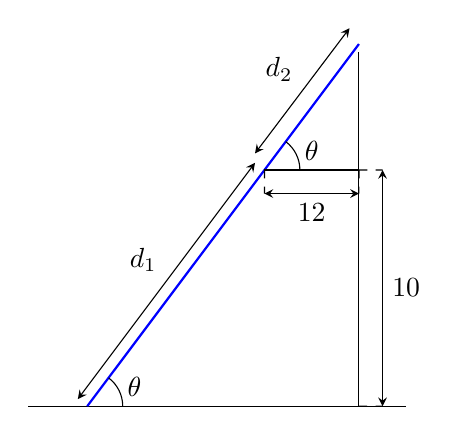
\begin{tikzpicture}[>=stealth, scale=0.3]
				\draw (0,0) -- (16,0) (14,0) -- (14,15);
				\coordinate (A) at (2.5,0); % Chân thang
				\coordinate (B) at (10,10); % Điểm chạm mái hiên
				\coordinate (C) at (14,15.33); % Ngọn thang chạm tường
				\coordinate (H) at (10,0); % Hình chiếu của B xuống đất
				\coordinate (K) at (14,10); % Hình chiếu của B vào tường
				\draw[thick, blue] (A) -- (C);
				% Vẽ mái hiên (đoạn nằm ngang)
				\draw (B) -- (K);
				% Kẻ đường gióng kích thước 10
				\draw[<->] (15,0) -- (15,10) node[midway, right] {$10$};
				\draw[dashed] (K) -- (15,10) (14,0) -- (15,0);
				% Kẻ đường gióng kích thước 12
				\draw[<->] (10,9) -- (14,9) node[midway, below] {$12$};
				\draw[dashed] (B) -- (10,9) (K) -- (14,9);
				\draw (4,0) arc (0:53:1.5);\node at (4.5,0.8) {$\theta$};
				\draw (11.5,10) arc (0:53:1.5);\node at (12,10.8) {$\theta$};
				\draw[<->] (2.1,0.3) -- (9.6,10.3) node[midway, above left] {$d_1$};
				\draw[<->] (9.6,10.7) -- (13.6,16) node[midway, above left] {$d_2$};
			\end{tikzpicture}
		}
		\noindent
		Ta có
		$$\begin{aligned}
			f'(\theta)=0 
			& \Leftrightarrow \dfrac{12\sin\theta}{\cos^2\theta}=\dfrac{10\cos\theta}{\sin^2\theta} \\
			& \Leftrightarrow \dfrac{\sin^3\theta}{\cos^3\theta}=\dfrac{10}{12} \\
			& \Leftrightarrow \tan^3\theta=\dfrac{5}{6} \\
			& \Leftrightarrow \tan\theta=\sqrt[3]{\dfrac{5}{6}} \\ 
			& \Leftrightarrow \theta=\theta_0\approx0{,}76 \, (\text{rad}).
		\end{aligned}$$
		Bảng biến thiên của $f(\theta)$
		\begin{center}
			
\begin{tikzpicture}[scale=1, >=stealth]
				\tkzTabInit[nocadre=false, lgt=1.2, espcl=2.5, deltacl=0.6]{$\theta$/1, $f'(\theta)$/0.6, $f(\theta)$/3}{$0$, $\theta_0$, $\dfrac{\pi}{2}$}
				\tkzTabLine{,-,0,+,}
				\tkzTabVar{+/, -/, +/}
			\end{tikzpicture}
		\end{center}
		Từ bảng biến thiên ta có $\min\limits_{\left(0;\dfrac{\pi}{2}\right)} f(\theta)=f\left(\theta_0\right)$ (m). \\
		Vậy độ dài ngắn nhất của chiếc thang cần thiết là $f\left(\theta_0\right)-\dfrac{1{,}2}{\sin\theta_0}\approx 29{,}3$ m.
	}
\end{ex}

\begin{ex}%[TT-ThieuHoa-ThanhHoa-L1-25-26]%[Vũ Nguyễn Hoàng Anh]%[0D0K2-5]
	Hai thí sinh $A$ và $B$ cùng tham gia một cuộc thi vấn đáp. Cán bộ coi thi đưa cho mỗi thí sinh một bộ câu hỏi gồm $10$ câu hỏi khác nhau, được đựng trong $10$ phong bì dán kín, có hình thức giống hệt nhau, mỗi phong bì đựng $1$ câu hỏi; thí sinh chọn $3$ phong bì để xác định câu hỏi của mình. Biết rằng bộ $10$ câu hỏi của các thí sinh là như nhau. Hai phong bì được gọi là giống nhau nếu chứa cùng một câu hỏi. Xác suất để $3$ phong bì $A$ chọn và $3$ phong bì $B$ chọn có ít nhất hai phong bì giống nhau là $\dfrac{a}{b}$ (trong đó $\dfrac{a}{b}$ là phân số tối giản và $a,b\in\mathbb{N}$). Tính $a^2+b^2$.
	
	\shortans{3721}
	\loigiai{
		Số cách để $A$ và $B$ chọn đúng hai phong bì giống nhau ($A$ và $B$ chọn $2$ phong bì giống nhau rồi  $A$ và $B$ lần lượt chọn $1$ phong bì khác với hai cái vừa chọn và khác nhau) là $\mathrm{C}^2_{10}\cdot \mathrm{C}^1_8\cdot \mathrm{C}^1_7$.\\
		Số cách để $A$ và $B$ chọn được ba phong bì giống nhau là $\mathrm{C}^3_{10}$.\\
		Suy ra xác suất cần tìm là $\dfrac{\mathrm{C}^2_{10}\cdot \mathrm{C}^1_8\cdot \mathrm{C}^1_7+\mathrm{C}^3_{10}}{\mathrm{C}^3_{10}\mathrm{C}^3_{10}}=\dfrac{11}{60}$.\\
		Do dó $a=11$, $b=60$ và $a^2+b^2=3\,721$.
	}
\end{ex}

\begin{ex}%[TT-ThieuHoa-ThanhHoa-L1-25-26]%[Vũ Nguyễn Hoàng Anh]%[1H8K7-6]
	\immini{
		Bác Bình có một chậu cảnh trồng hoa hình chóp cụt tứ giác đều với chiều cao $30$ cm, cạnh đáy lần lượt là $20$ cm và $40$ cm.
	Bác Bình đổ đất vào chậu để tiến hành trồng, chiều cao của đất bằng $ \dfrac{2}{3} $ chiều cao của chậu. Tính thể tích lượng đất bác Bình đã đổ vào chậu theo dm$^3$ (làm tròn kết quả đến hàng phần mười). 
	}{
		\begin{tikzpicture}[line cap=round, line join=round,font=\footnotesize,>=stealth, scale=0.7]
			\tikzset{label style/.style={font=\footnotesize}}
			\clip (-0.5,-2) rectangle (5.5,1.8);
			\def\a{4}
			\def\h{4.5}
			\path 	(0:0) coordinate (A)
			++(0:\a) coordinate (D)
			++(50:\a/2) coordinate (C)
			($(A)+(C)-(D)$) coordinate (B)
			(intersection of A--C and B--D) coordinate (O)
			($(O)-(90:\h)$) coordinate (S);
			\foreach\x in {A,B,C,D}{
				\path ($(S)!0.5!(\x)$) coordinate (\x')
				($(\x)!1/3!(\x')$) coordinate (\x1);}
			\path (intersection of C1--B1 and C--D) coordinate (a)
			(intersection of A1--B1 and A--D) coordinate (b); 
			\fill[brown!30] (A1)--(B1)--(C1)--(D1)
			(A')--(A1)--(D1)--(D')
			(D')--(C')--(C1)--(D1);
			\draw (a)--(B1)--(b);
			\draw (A')--(D')--(C')
			(A)--(D)--(C)--(B)--(A)--(A') (C)--(C') (D)--(D') (A1)--(D1)--(C1) (B1)--(B);
			\draw[dashed] (C')--(B')--(A') (C1)--(a) (b)--(A1) (B')--(B1);
		\end{tikzpicture}
	}
	\shortans{14,5}
	\loigiai{
		Phần đất trong chậu cũng tạo thành một khối chóp cụt đều có chiều cao là $\dfrac{2}{3}\cdot 30=20$ cm và có một đáy có cạnh là $20$ cm, một đáy có cạnh là $\dfrac{20+2\cdot 40}{3}=\dfrac{100}{3}$ cm. Do đó thể tích khối đất đã đổ vào là
		\[ \frac{1}{3}\cdot 20\left[20^2+\left(\frac{100}{2}\right)^2+20\cdot \frac{100}{3}\right]=\frac{392\,000}{27}\text{ cm}^3\approx 14{,}5\text{ dm}^3. \] 
	}
\end{ex}


\Closesolutionfile{ans}

% \indapan{4}{ans/ans-TT-ThieuHoa-ThanhHoa-L1-25-26}


>>>>>>> 33890a9ce1cfbd3079ed36a93e836cf3ef1fde30
